% Judul dokumen
\title{Buku Tugas Akhir ITS}
\author{Bahaduri, Dimas Nazli}

% Pengaturan ukuran teks dan bentuk halaman dua sisi
\documentclass[12pt,twoside]{report}

% Pengaturan ukuran halaman dan margin
\usepackage[a4paper,top=30mm,left=30mm,right=20mm,bottom=25mm]{geometry}

% Pengaturan ukuran spasi
\usepackage[singlespacing]{setspace}

% Pengaturan format bahasa
\usepackage[indonesian]{babel}

% Pengaturan detail pada file PDF
\usepackage[pdfauthor={\@author},bookmarksnumbered,pdfborder={0 0 0}]{hyperref}

% Pengaturan jenis karakter
\usepackage[utf8]{inputenc}

% Pengaturan pewarnaan
\usepackage[table,xcdraw]{xcolor}

% Pengaturan kutipan artikel
\usepackage{apacite}

% Package lainnya
\usepackage{changepage}
\usepackage{enumitem}
\usepackage{eso-pic}
\usepackage{etoolbox}
\usepackage{graphicx}
\usepackage{lipsum}
\usepackage{lmodern}
\usepackage{longtable}
\usepackage{tabularx}
\usepackage{wrapfig}

% Definisi untuk "Hati ini sengaja dikosongkan"
\patchcmd{\cleardoublepage}{\hbox{}}{
  \thispagestyle{empty}
  \vspace*{\fill}
  \begin{center}\textit{[Halaman ini sengaja dikosongkan]}\end{center}
  \vfill}{}{}

% Pengaturan penomoran halaman
\usepackage{fancyhdr}
\fancyhf{}
\renewcommand{\headrulewidth}{0pt}
\pagestyle{fancy}
\fancyfoot[RE,RO]{\thepage}
\patchcmd{\chapter}{plain}{fancy}{}{}
\patchcmd{\chapter}{empty}{plain}{}{}

% Pengaturan format judul bab
\usepackage{titlesec}
\titleformat{\chapter}[display]{\bfseries\Large}{BAB \centering\Roman{chapter}}{0ex}{\vspace{0ex}\centering}
\titleformat{\section}{\bfseries\large}{\MakeUppercase{\thesection}}{1ex}{\vspace{1ex}}
\titleformat{\subsection}{\bfseries\large}{\MakeUppercase{\thesubsection}}{1ex}{}
\titleformat{\subsubsection}{\bfseries\large}{\MakeUppercase{\thesubsubsection}}{1ex}{}
\titlespacing{\chapter}{0ex}{0ex}{4ex}
\titlespacing{\section}{0ex}{1ex}{0ex}
\titlespacing{\subsection}{0ex}{0.5ex}{0ex}
\titlespacing{\subsubsection}{0ex}{0.5ex}{0ex}

% Pengaturan format potongan kode
\usepackage{listings}
\definecolor{comment}{RGB}{0,128,0}
\definecolor{string}{RGB}{255,0,0}
\definecolor{keyword}{RGB}{0,0,255}
\lstdefinestyle{codestyle}{
  commentstyle=\color{comment},
  stringstyle=\color{string},
  keywordstyle=\color{keyword},
  basicstyle=\footnotesize\ttfamily,
  numbers=left,
  numberstyle=\tiny,
  numbersep=5pt,
  frame=lines,
  breaklines=true,
  prebreak=\raisebox{0ex}[0ex][0ex]{\ensuremath{\hookleftarrow}},
  showstringspaces=false,
  upquote=true,
  tabsize=2,
}
\lstset{style=codestyle}

% Isi keseluruhan dokumen
\begin{document}

  % Sampul luar Bahasa Indonesia
  \newcommand\covercontents{sampul/konten-id.tex}
  \AddToShipoutPictureBG*{
  \AtPageLowerLeft{
    % Ubah nilai berikut jika posisi horizontal background tidak sesuai
    \hspace{-3.5mm}

    % Ubah nilai berikut jika posisi vertikal background tidak sesuai
    \raisebox{0mm}{
      
\includegraphics[width=\paperwidth,height=\paperheight]{sampul/gambar/sampul-luar2.png}
    }
  }
}

% Menyembunyikan nomor halaman
\thispagestyle{empty}

% Pengaturan margin untuk menyesuaikan konten sampul
\newgeometry{
  top=55mm,
  left=30mm,
  right=20mm,
  bottom=25mm
}

\begin{flushleft}
  % Pemilihan font sans serif
  \sffamily

  % Pemilihan warna font putih
  \color{white}

  % Pemilihan font bold
  % \fontseries{bx}
  \selectfont

  \input{\covercontents}

\end{flushleft}

\restoregeometry


  % Atur ulang penomoran halaman
  \setcounter{page}{1}

  % Sampul dalam Bahasa Indonesia
  \renewcommand\covercontents{sampul/konten-id.tex}
  \AddToShipoutPictureBG*{
  \AtPageLowerLeft{
    % Ubah nilai berikut jika posisi horizontal background tidak sesuai
    \hspace{-3.5mm}

    % Ubah nilai berikut jika posisi vertikal background tidak sesuai
    \raisebox{0mm}{
      
\includegraphics[width=\paperwidth,height=\paperheight]{sampul/gambar/sampul-dalam2.png}
    }
  }
}

% Menyembunyikan nomor halaman
\thispagestyle{empty}

% Pengaturan margin untuk menyesuaikan konten sampul
\newgeometry{
  top=65mm,
  left=30mm,
  right=20mm,
  bottom=25mm
}

\begin{flushleft}

  % Pemilihan font sans serif
  \sffamily

  % Pemilihan font bold
  % \fontseries{bx}
  \selectfont

  \input{\covercontents}

\end{flushleft}

\restoregeometry

  \clearpage
  \cleardoublepage

  % Sampul dalam Bahasa Inggris
  \renewcommand\covercontents{sampul/konten-en.tex}
  \AddToShipoutPictureBG*{
  \AtPageLowerLeft{
    % Ubah nilai berikut jika posisi horizontal background tidak sesuai
    \hspace{-3.5mm}

    % Ubah nilai berikut jika posisi vertikal background tidak sesuai
    \raisebox{0mm}{
      
\includegraphics[width=\paperwidth,height=\paperheight]{sampul/gambar/sampul-dalam2.png}
    }
  }
}

% Menyembunyikan nomor halaman
\thispagestyle{empty}

% Pengaturan margin untuk menyesuaikan konten sampul
\newgeometry{
  top=65mm,
  left=30mm,
  right=20mm,
  bottom=25mm
}

\begin{flushleft}

  % Pemilihan font sans serif
  \sffamily

  % Pemilihan font bold
  % \fontseries{bx}
  \selectfont

  \input{\covercontents}

\end{flushleft}

\restoregeometry

  \cleardoublepage

  % Pengaturan ukuran indentasi paragraf
  \setlength{\parindent}{2em}

  % Pengaturan ukuran spasi paragraf
  \setlength{\parskip}{1ex}

  % Lembar pengesahan
  \begin{center}
	\large
  \textbf{LEMBAR PENGESAHAN}
\end{center}

% Menyembunyikan nomor halaman
\thispagestyle{empty}

\begin{center}
  % Ubah kalimat berikut dengan judul tugas akhir
  \textbf{\emph{ETHER WALLET} MENGGUNAKAN \emph{ETHEREUM} BERBASIS \emph{PROOF OF STAKE} UNTUK VALIDASI TRANSAKSI}
\end{center}

\begingroup
  % Pemilihan font ukuran small
  \small
  
  \vspace{3ex}

  \begin{center}
    \textbf{PROPOSAL TUGAS AKHIR}
    \\Diajukan untuk memenuhi salah satu syarat
    \\memperoleh gelar Sarjana pada
    \\Program Studi S-1 Teknik Komputer
    \\Departemen Teknik Komputer
    \\Fakultas Teknologi Elektro dan Informatika Cerdas
    \\Institut Teknologi Sepuluh Nopember
  \end{center}

  \vspace{3ex}

  \begin{center}
    % Ubah kalimat berikut dengan nama dan NRP mahasiswa
    Oleh: Dimas Nazli Bahaduri
    \\NRP. 0721 18 4000 0060
  \end{center}

  \vspace{3ex}

  % \begin{center}
  % Ubah kalimat-kalimat berikut dengan tanggal ujian dan periode wisuda
  %   Tanggal Ujian : 1 Juni 2021\\
  %   Periode Wisuda : September 2021
  % \end{center}

  \begin{center}
    Disetujui oleh Tim Penguji Tugas Akhir:
  \end{center}

  \vspace{4ex}

  \begingroup
    % Menghilangkan padding
    \setlength{\tabcolsep}{0pt}

    \noindent
    \begin{tabularx}{\textwidth}{X l}
      % Ubah kalimat-kalimat berikut dengan nama dosen pembimbing pertama
      1. Mochamad Hariadi, S.T., M.Sc., Ph.D.          & Pembimbing I \\
      NIP: 196912091997031002        & ................................... \\
      &  \\
      &  \\
      % Ubah kalimat-kalimat berikut dengan nama dosen pembimbing kedua
      2. Dr. Supeno Mardi Susiki Nugroho, S.T., M.T.     & Pembimbing II \\
      NIP: 197003131995121001        & ................................... \\
      &  \\
      &  \\
      % Ubah kalimat-kalimat berikut dengan nama dosen penguji pertama
    \end{tabularx}
  \endgroup

  \vspace{12ex}

  % \begin{center}
  %   % Ubah kalimat berikut dengan jabatan kepala departemen
  %   Mengetahui, \\
  %   Kepala Departemen Teknik Dirgantara FTD - ITS \\

  %   \vspace{8ex}

  %   % Ubah kalimat-kalimat berikut dengan nama dan NIP kepala departemen
  %   \underline{Dr. Leonardo Da Vinci, S.T., M.T.} \\
  %   NIP. 14520415 151905 1 001
  % \end{center}

  \begin{center}
    \textbf{SURABAYA\\Mei, 2022}
  \end{center}
\endgroup

  \cleardoublepage

  % Pernyataan keaslian
  \begin{center}
  \large
  \textbf{PERNYATAAN ORISINALITAS}
\end{center}

% Menyembunyikan nomor halaman
\thispagestyle{empty}

\vspace{2ex}

% Ubah paragraf-paragraf berikut sesuai dengan yang ingin diisi pada pernyataan keaslian

\noindent Yang bertanda tangan dibawah ini:

\noindent\begin{tabularx}{\textwidth}{X X l}
  & \\
  Nama Mahasiswa / NRP &: Dimas Nazli Bahaduri / 07211840000060 \\
  Departemen &: Departemen Teknik Komputer\\
  Dosen Pembimbing &: Mochamad Hariadi, ST., M.Sc., Ph.D. \\
  & Dr. Supeno Mardi Susiki Nugroho, ST., M.T. \\
\end{tabularx}

Dengan ini menyatakan bahwa Tugas Akhir dengan judul "\emph{Ether Wallet} Menggunakan \emph{Ethereum} Berbasis \emph{Proof of Stake} Untuk Validasi Transaksi" adalah hasil karya sendiri, berfsifat orisinal, dan ditulis dengan mengikuti kaidah penulisan ilmiah.

Bilamana di kemudian hari ditemukan ketidaksesuaian dengan pernyataan ini, maka saya bersedia menerima sanksi sesuai dengan ketentuan yang berlaku di Institut Teknologi Sepuluh Nopember.

\vspace{8ex}

\noindent\begin{tabularx}{\textwidth}{X l}
  % Ubah kalimat berikut sesuai dengan tempat, bulan, dan tahun penulisan
  & Surabaya,  2022\\
  & \\
  Mengetahui & \\
  Dosen Pembimbing & Mahasiswa\\
  & \\
  & \\
  & \\
  & \\
  & \\
  Mochamad Hariadi, ST., M.Sc., Ph.D. & Dimas Nazli Bahaduri \\
  NIP. 196912091997031002 & NRP. 0721 18 4000 0060\\
\end{tabularx}
  \cleardoublepage

  % Nomor halaman pembuka dimulai dari sini
  \pagenumbering{roman}

  % Abstrak Bahasa Indonesia
  \begin{center}
  \large\textbf{ABSTRAK}
\end{center}

\addcontentsline{toc}{chapter}{ABSTRAK}

\vspace{2ex}

\begingroup
  % Menghilangkan padding
  \setlength{\tabcolsep}{0pt}

  \noindent
  \begin{tabularx}{\textwidth}{l >{\centering}m{2em} X}
    % Ubah kalimat berikut dengan nama mahasiswa
    Nama Mahasiswa    &:& Dimas Nazli Bahaduri \\

    % Ubah kalimat berikut dengan judul tugas akhir
    Judul Tugas Akhir &:&	\emph{Ether Wallet} Menggunakan \emph{Ethereum} Berbasis \emph{Proof of Stake} Untuk Validasi Transaksi \\

    % Ubah kalimat-kalimat berikut dengan nama-nama dosen pembimbing
    Pembimbing        &:& 1. Mochamad Hariadi, ST., M.Sc., Ph.D. \\
  &:& 2. Dr. Supeno Mardi Susiki Nugroho, ST., MT.
  \end{tabularx}
\endgroup

% Ubah paragraf berikut dengan abstrak dari tugas akhir
Pada penelitian ini kami mengajukan penelitian yang memanfaatkan perkembangan \emph{Ethereum} sebagai salah satu solusi perbankan yaitu dompet digital. Bagian perbankan mengalami perkembangan dengan mengadopsi dompet digital yang dinilai cukup bagus bagi konsumen karena meminimalisir transaksi tak tercatat. Sebagai solusi terpusatnya digunakanlah \emph{Blockchain Ethereum} sebagai sistem transaksi utama. \emph{Ethereum} ini mengadopsi sistem informasi terdistribusi yang mana mengharuskan setiap audit informasi dibagikan ke semua pengguna yang terhubung. Alhasil dengan sistem informasi seperti ini, segala transaksi dan akses informasi bisa terlihat ke semua node yang membuat sulit untuk diubah. Nantinya dengan mengadopsi \emph{Ethereum} ke dalam dompet digital baru diharapkan bisa mengeliminasi masalah yang mungkin ditemui dari dompet konvensional dan memberikan opsi baru bagi pengguna konsumen di Indonesia untuk bertransaksi tanpa batas. Penelitian ini akan menjalankan proses transaksi yang diawali dengan permintaan untuk melakukan transaksi. Ketika proses transaksi dimulai akan dilakukan verifikasi data transaksi dari penerima dan mengirim. Setelah transaksi terverifikasi, selanjutkan proses validasi dari node – node tergabung dengan jaringan \emph{Ethereum}. Validasi ini akan menggunakan konsensus/kesepakatan \emph{Proof of Stake} yang mana menganalisa apakah benar pengirim mempunyai sejumlah nominal yang akan dikirimkan. Kemudian jika validasi sudah mencapai ambang batas,sejumlah nominal tercantum dalam transaksi akan dikirimkan dari pengirim ke penerima. Maka proses transaksi tersebut selesai. Dari hasil sementara yang didapatkan, implementasi sebaagian fitur dompet digital yaitu deteksi deposit ke \emph{Ether} dan deteksi pemilik dompet digital. Dari hasil sementara didapati proses deposit bisa uang dapat diselesaikan dalam waktu 13.212 detik di jaringan Testnet Kintsugi dan Kiln

% Ubah kata-kata berikut dengan kata kunci dari tugas akhir
Kata Kunci: Dompet digital, \emph{Ethereum}, \emph{Proof of Stake, Blockchain}. 

  \cleardoublepage

  % Abstrak Bahasa Inggris
  \begin{center}
  \large\textbf{ABSTRACT}
\end{center}

\addcontentsline{toc}{chapter}{ABSTRACT}

\vspace{2ex}

\begingroup
  % Menghilangkan padding
  \setlength{\tabcolsep}{0pt}

  \noindent
  \begin{tabularx}{\textwidth}{l >{\centering}m{3em} X}
    % Ubah kalimat berikut dengan nama mahasiswa
    \emph{Name}     &:& Dimas Nazli Bahaduri \\

    % Ubah kalimat berikut dengan judul tugas akhir dalam Bahasa Inggris
    \emph{Title}    &:& \emph{Ether Wallet using Ethereum based on Proof of Stake for Validating Transaction} \\

    % Ubah kalimat-kalimat berikut dengan nama-nama dosen pembimbing
    \emph{Advisors} &:& 1. Mochamad Hariadi, ST., M.Sc., Ph.D. \\
  &:& 2. Dr. Supeno Mardi Susiki Nugroho, ST., MT.
  \end{tabularx}
\endgroup

% Ubah paragraf berikut dengan abstrak dari tugas akhir dalam Bahasa Inggris
\emph{In this research, we propose a study that uses Ethereum as a banking solution, namely a digital wallet. The banking department has developed by adopting a digital wallet which is considered good for consumers because it minimizes recorded transactions. As a solution, Ethereum is used as the main transaction system. This Ethereum adopts a distributed information system which requires that every audit information be shared with all connected users. As a result, with an information system like this, all transactions and information access can be seen to all nodes which makes it difficult to change. Later, by adopting Ethereum into a new digital wallet, it is hoped that it will eliminate problems that may be encountered from conventional wallets and provide new options for consumer users in Indonesia to transact without limits. This research will run a transaction process that starts with a request to make a transaction. When the transaction process starts, verification of transaction data from the recipient and delivery will be carried out. After the transaction is verified, continue the validation process from the nodes joined to the Ethereum network. This validation will use the Proof of Stake convention/agreement which analyzes whether the sender actually has the number to send. Then if the validation has reached the threshold, a nominal amount is listed in the transaction that will be sent from the sender to the recipient. Then the transaction process is complete. From the temporary results obtained, the implementation of some digital wallet features, namely detection of deposits to Ether and detection of digital wallet owners. From the temporary results the transaction can be completed within 13,212 seconds.}

% Ubah kata-kata berikut dengan kata kunci dari tugas akhir dalam Bahasa Inggris
\emph{Keywords}:\emph{Digital Wallet} ,\emph{Ethereum} ,\emph{Proof of Stake}  ,\emph{Blockchain}.

  \cleardoublepage

  % Kata pengantar
  \begin{center}
  \Large
  \textbf{KATA PENGANTAR}
\end{center}

\addcontentsline{toc}{chapter}{KATA PENGANTAR}

\vspace{2ex}

% Ubah paragraf-paragraf berikut dengan isi dari kata pengantar

Puji dan syukur kehadirat penyusun sampaikan kepada Allah SWT. karena atas limpahan berkat, rahmat, dan hidayah-Nya penulis dapat menyelesaikan penelitian berjudul \textbf{ \emph{Ether Wallet} Menggunakan \emph{Ethereum} Berbasis \emph{Proof of Stake} untuk Validasi Transaksi} ini tepat waktu.

Penelitian ini disusun dalam rangka pemenuhan bidang riset di Departemen Teknik Komputer, serta digunakan sebagai persyaratan menyelesaikan pendidikan S1. Penelitian ini dapat terselesaikan tidak lepas dari bantuan berbagai pihak. Oleh karena itu, penulis mengucapkan terima kasih kepada:

\begin{enumerate}[nolistsep]

  \item Keluarga, Ibu, Abang dan Kakak tercinta yang telah memberikan dukungan moril maupun dukungan material dalam menyelesaikan penelitian ini. 

  \item Bapak Supeno Mardi Susiki Nugroho, S.T., M.T. selaku Kepala Departemen Teknik Komputer, Fakultas Teknologi Elektro dan Informatika Cerdas (FTEIC), Institut Teknologi Sepuluh Nopember.

  \item Bapak Mochamad Hariadi, S.T., M.Sc., Ph.D. selaku dosen pembimbing I dan Bapak Dr. Supeno Mardi Susiki Nugroho, S.T., M.T. selaku  dosen pembimbing II yang memberikan arahan dan petuah selama mengerjakan penelitian tugas akhir ini. 

 \item Bapak dan ibu dosen pengajar Departemen Teknik Komputer, atas pengajaran, bimbingan, serta perhatian yang diberikan selama ini.

 \item Secara khusus penulis mengucapkan terima kasih kepada teman teman satu bimbingan terutama Rizqullah dan Ananta, yang telah berbagi ilmu dan pikirannya selama ini. Tiada dirimu, diriku hanya diam termenung.

 \item Teman-teman dari seluruh kalangan yang tidak bisa penulis sebutkan satu per satu namun tidak membuat penulis lupa dukungan yang terus kalian suguhkan baik melalui kesenangan permainan maupun curhatan melantur di tengah malam.	 

\end{enumerate}

Sebagaimana pepatah berkata "Tiada Gading yang Tak Retak", maka dari itu penulis mengharapkan kritik dan saran yang membangun. Akhir kata, semoga penelitian ini dapat digunakan semestinya dan bermanfaat bagi semua. Amin. 

\begin{flushright}
  \begin{tabular}[b]{c}
    % Ubah kalimat berikut dengan tempat, bulan, dan tahun penulisan
    Surabaya, Mei 2022\\ 
    \\
    \\
    \\
    \\
    % Ubah kalimat berikut dengan nama mahasiswa
    Dimas Nazli Bahaduri
  \end{tabular}
\end{flushright}

  \cleardoublepage

  % Daftar isi
  \renewcommand*\contentsname{DAFTAR ISI}
  \addcontentsline{toc}{chapter}{\contentsname}
  \tableofcontents
  \cleardoublepage

  % Daftar gambar
  \renewcommand*\listfigurename{DAFTAR GAMBAR}
  \addcontentsline{toc}{chapter}{\listfigurename}
  \listoffigures
  \cleardoublepage

  % Daftar tabel
  \renewcommand*\listtablename{DAFTAR TABEL}
  \addcontentsline{toc}{chapter}{\listtablename}
  \listoftables
  \cleardoublepage

  % Nomor halaman isi dimulai dari sini
  \pagenumbering{arabic}

  % Bab 1 pendahuluan
  \chapter{PENDAHULUAN}
\label{chap:pendahuluan}

% Ubah bagian-bagian berikut dengan isi dari pendahuluan

\section{Latar Belakang}
\label{sec:latarbelakang}

Di era industri 4.0 dan perkembangan 5G di Indonesia, saat ini Indonesia sedang bersiap menjadi sebuah negara yang berkembang untuk mengadopsi teknologi untuk menunjang sektor industri dan sektor bisnis. Sektor bisnis dan sektor industri di Indonesia sedang mengalami pemulihan yang ditandai dengan beberapa program nasional pemulihan pasca COVID-19. Program pemulihan ekonomi pasca COVID-19 ini bertujuan untuk mempersiapkan Indonesia bersaing di kancah dunia. Dalam proses perkembangan Indonesia untuk bersaing di panggung dunia, tentu diiringi dengan perkembangan teknologi perbankan yaitu pembuatan dompet digital. \\
Serupa dengan dompet pada umumnya yang menyimpan uang, dompet digital ini adalah aplikasi untuk menyimpan uang, melakukan transaksi, kirim uang, dan sebagainya. Dompet digital ini banyak digunakan untuk kegiatan tersebut dan melansir dari Kontan.co.id, kegiatan dan transaksi di salah satu dompet digital mengalami kenaikan hingga 91\% dan MAU sebesar 73\%. Ini bisa jadi menandakan pertumbuhan ekonomi dan bisnis di Indonesia. Dompet digital ini juga menyediakan fitur masing-masing. Namun dari segelintir fitur ini dompet digital yang ada di Indonesia belum bisa menjangkau transfer ke luar negeri. Padahal beberapa produk Indonesia sudah mulai dilirik di beberapa negara tetangga. \\
Seperti yang diketahui bahwa Indonesia sedang bersiap menuju pemulihan pasca COVID-19 dan diperlukan fasilitas penunjang kegiatan ekonomi berbasis teknologi. Aplikasi dari teknologi yang telah ada untuk menjamin kenyamanan dan keamanan kegiatan bisnis. Teknologi harus mampu mengatasi beberapa aspek dasar dalam kegiatan transaksi mancanegara.\\
Terdapat teknologi untuk mendukung kebutuhan ini yaitu \emph{Blockchain}. Teknologi ini berdasarkan transfer file peer-to-peer yang aman. Dan saat ini sudah banyak jenis \emph{Blockchain} yang digunakan di dunia mulai dari \emph{Bitcoin, Ethereum, Solana, hingga Pancakeswap}. Semua \emph{Blockchain} ini punya implementasi mulai dari pengiriman pesan sederhana, \emph{public ledger}, hingga dompet digital. 

\section{Permasalahan}
\label{sec:permasalahan}

Berdasarkan pendahuluan diatas,dapat ditarik sebuah permasalahan yaitu perlu adanya sebuah alat transaksi yang mengadopsi sistem informasi yang terdistribusi atau \emph{Blockchain}. Alat transaksi tersebut adalah dompet digital yang berbasis \emph{Ethereum} menggunakan konsensus/kesepakatan \emph{Proof of Stake} sebagai cara untuk validiasi transaksinya.

\section{Batasan Masalah}
\label{sec:batasanmasalah}

Untuk memfokuskan permasalahan yang diangkat maka dilakukan pembatasan masalah. Berikut batasan-batasan masalah tersebut diantaranya adalah:

\begin{enumerate}[nolistsep]

  \item \emph{Blockchain} beserta \emph{Cryptocurrencies} yang digunakan dalam penelitian ini adalah \emph{Ethereum} dan \emph{Ether} beserta turunan dari Ether tersebut.
  \item Jenis jaringan yang digunakan adalah jaringan \emph{testnet} yang tersedia
  \item Sistem dompet hanya akan melakukan fitur berupa mengirim uang, mendeteksi akun, dan mengirimkan sejumlah \emph{Ether}
  \item Aplikasi dompet digital akan berbentuk website.
  \item Aplikasi penghubung antara \emph{Ethereum} dan aplikasi dompet digital yaitu \emph{Metamask}.

\end{enumerate}

\section{Tujuan}
\label{sec:Tujuan}

Dari penelitian yang akan dilakukan kali ini, penulis ingin mencapai tujuan yaitu membuktikan penggunaan \emph{Blockchain Ethereum} sebagai sistem alat transaksi dengan mengirimkan sejumlah \emph{Ether} antar pengguna dan mengetahui nilai optimal gas yang digunakan untuk transaksi sehari-hari.

\section{Manfaat}
\label{sec:manfaat}

Manfaat dari penelitian ini adalah membuat sebuah sistem dompet digital yang menggunakan \emph{Ethereum} yang bisa digunakan untuk transaksi digital di Indonesia.

% Format Buku TA baru, ga pake sistematika penulisan

% \section{Sistematika Penulisan}
% \label{sec:sistematikapenulisan}

% Laporan penelitian tugas akhir ini terbagi menjadi \lipsum[1][1-3] yaitu:

% \begin{enumerate}[nolistsep]

%   \item \textbf{BAB I Pendahuluan}

%   Bab ini berisi \lipsum[2][1-5]

%   \vspace{2ex}

%   \item \textbf{BAB II Tinjauan Pustaka}

%   Bab ini berisi \lipsum[3][1-5]

%   \vspace{2ex}

%   \item \textbf{BAB III Desain dan Implementasi Sistem}

%   Bab ini berisi \lipsum[4][1-5]

%   \vspace{2ex}

%   \item \textbf{BAB IV Pengujian dan Analisa}

%   Bab ini berisi \lipsum[5][1-5]

%   \vspace{2ex}

%   \item \textbf{BAB V Penutup}

%   Bab ini berisi \lipsum[6][1-5]

% \end{enumerate}

  \cleardoublepage

  % Bab 2 tinjauan pustaka
  \chapter{TINJAUAN PUSTAKA}
\label{chap:tinjauanpustaka}

% Ubah bagian-bagian berikut dengan isi dari tinjauan pustaka
\section{Penelitian Terdahulu}
\label{sec:penelitianterdahulu}

Pada penelitian yang telah dilakukan oleh Reza Putra Pradana bertajuk \emph{Sistem Transaksi Antar Player Pada Game Multiplayer Wisata Bromo Menggunakan Blockchain} dikemukakan bahwa transaksi digital bisa menggunakan \emph{Ethereum} dengan harga per transaksi Rp.471 dengan kecepatan antara 3 - 30 detik \cite{pradana2020}. Pada penelitian yang dilakukan oleh Reza Putra Pradana, dilakukan penelitian dan penjelasan mengenai penggunaan \emph{Blockchain Ethereum} untuk sistem pembayaran di dalam game yang dia buat. Dalam game tersebut dibuat menggunakan Game Engine Unity dan sistem pembayaran yaitu Ethereum. Dengan menggunakan Unity tersebut dibuat sistem game role play gaming yang mana pengguna berperan sebagai pengunjung/wisatawan yang mengunjungi daerah Gunung Bromo. Dalam kawasan Gunung Bromo tersebut terdapat kegiatan yang bisa dilakukan di dalam kawasan mulai dari masuk ke kawasan sekitar kawah gunung, membeli makan, membeli tiket, hingga menyewa kendaraan. Semua interaksi di dalam kawasan Gunung Bromo dilakukan melalui interaksi NPC dan menggunakan mata uang Ether. Untuk pengujian sistem transaksi menggunakan \emph{provider} internet mobile Indonesia, dan mendapatkan hasil performa latensi yang diterima antara perangkat pengunjung dengan perangkat NPC berkisar antara 61ms - 144ms. Angka ini tergolong memiliki performa cukup untuk digunakan sehari hari. Kemudian performa sistem Ethereum yang digunakan menelan biaya berkisar antara Rp300.000,- hingga Rp3.000.000,- per bulan dengan rincian Rp300,- hingga Rp3.000,- per transaksi x 1000 transaksi per bulan.

\section{Validasi}
\label{sec:validasi}

Melansir dari KBBI daring, validasi adalah sebuah kegiatan untuk melakukan pengujian kebenaran atas sesuatu. Dalam lingkup Ethereum validasi adalah serangkaian kegiatan untuk menguji kebenaran suatu transaksi yang akan dilakukan. Pengujian kebenaran data suatu transaksi dilakukan agar tidak terjadi kesalahan data pada suatu transaksi. Kesalahan yang dimaksud bisa terjadi dari luar sistem maupun dalam sistem. Apabila terjadi kesalahan data bisa membaut suatu transaksi tidak terjadi. Kesalahan data internal yang biasa terjadi adalah kesalahan penyediaan dan perhitungan gas. Sedangkan dari luar sistem bisa saja ada upaya interupsi transaksi. Interupsi interaksi ini bisa berupa serangan 51\% / 51\% attack di suatu sistem Ethereum. Dalam arsitektur Ethereum, proses pengujian kebenaran data yang dikirim (validasi) menggunakan sebuah  kesepakaran yaitu kesepakatan yang biasa disebut konsensus. Konsensus ini memungkinkan validasi sebuah data menggunakan tenaga komputer lainnya yang telah tergabung dengan berbagai syarat dari Ethereum itu sendiri.

\section{Kriptografi}
\label{sec:kriptografi}

Kriptografi adalah sebuah cara untuk mengamankan informasi yang dikirimkan oleh pengirim kepada penerima. Kriptografi memiliki peran dalam keamanan siber terutama dalam kerahasiaan inform si yang dikirim. Kerahasiaan informasi ini menjamin data dikirimkan tidak diubah selama dalam pengiriman dari pengirim ke penerima \cite{stallings1999cryptography}. Kriptografi mempunyai tujuang sebagai metode untuk mengenkripsi dan mendekripsi informasi yang dikirim dengan beberapa standar. Dalam Ethereum, kriptografi digunakan sebagai standar pembuatan blok baru yang telah divalidasi.  

\subsection{Fungsi Hash}
\label{subsec:hashfunction}

Fungsi hash adalah sebuah standar kriptografi yang mengenkripsi informasi yang dikirimkan dengan menggunakan matematika untuk memadatkan informasi yang dikirim dan menjadikannya satu potong informasi tetap yang utuh \cite{stallings1999cryptography}. Dalam praktiknya fungsi hash akan memproses informasi yang sangat banyak yang akan dikirim kemudian akan mengeluarkan nilai hash yang mempunyai jumlah tetap. Ini artinya fungsi hash memangkas jumlah data yang dikirim setelah di enkripsi dan selanjutnya dikirim dan di-dekripsikan oleh penerima. Apabila jumlah data yang dikirimkan sejulah 512bit maka apabila dilakukan fungsi hash akan tereduksi menjadi sekitar 160bit. Hasil dari fungsi hash ini akan terdiri atas kombinasi angka, huruf, dan simbol. Sedikit perbedaan informasi yang dienkripsi fungsi hash, maka hasil yang didapatkan akan menjadi berbeda sama sekali. Namun dalam praktiknya fungsi hash ini memerlukan banyak komputasi dan data yang bisa diproses pun dipecah menjadi beberapa bagian kecil.Karena hal ini fungsi hash digunakan di beberapa aplikasi saja. Dan dalam upaya menaikkan performa ini tercipta suatu fungsi hash yaitu SHA (\emph{Secure Hash Algorithm}).

\subsection{SHA (\emph{Secure Hash Algorithm})}
\label{subsec:sha}

SHA adalah salah satu jenih fungsi hash yang saat ini banyak digunakan sebagai tanda unik untuk mengetahui bahwa integritas suatu informasi. Dalam upaya untuk memecahkan informasi yang telah melalui fungsi hash, perlu dilakukan 'tenaga paksa' yang mana pada konteksnya berupaya mencocokkan suatu hasil output dengan input satu per satu dan dicoba secara berulang \cite{stallings1999cryptography}. SHA ditemukan oleh NIST (\emph{National Institute of Standards and Technology}) yang pada awalnya dapat mereduksi 512 bit menjadi 160 bit. Kemudian SHA pertama (SHA-0) terus dikembangkan dan terjadi beberapa iterasi hingga menjadi SHA-2 yang saat ini banyak digunakan.
\\
\begin{figure}
	\centering
	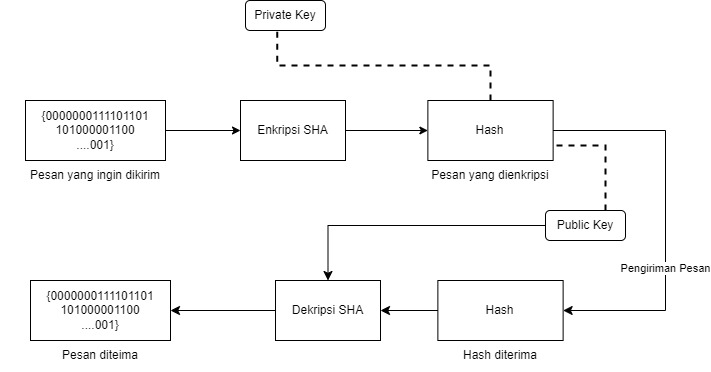
\includegraphics[scale=0.5]{gambar/sha.jpg}
	\caption{Ilustrasi SHA}
	\label{fig:shaillustrated}
\end{figure}
\\
Dalam praktiknya, SHA melakukan enkripsi dengan mengubah pesan yang ada menjadi angka dan huruf acak. Dalam proses enkripsinya akan diciptakan dua buah rangkaian kunci yaitu kunci publik dan kunci privat. Setelah enkripsi pesan selesai, ukuran pesan tereduksi dan menghasilkan kunci publik dan kunci privat. Pada kunci privat akan menjadi kunci yang krusial dalam menandakan pesan yang kita kirim. Kunci privat digunakan sebagai 'tanda tangan' kita dalam pesan yang terenkripsi. Kemudian kunci public bisa diberikan kepada penerima pesan sebagai autentikasi pesan yang kita enkripsi di awal adalah pesan sama yang telah diterima. Sedangkan kunci privat digunakan sebagai 'bon' bahwa kita telah melakukan SHA.Selanjutnya di sisi penerima pesan didekripsi sambil dicocokkan dengan kunci publik yang diberikan. Apabila kunci publik dengan pesan tidak cocok, maka pesan yang terenkripsi telah berubah dalam pengiriman. Apabila dalam proses enkripsi pesan yang dienkripsi mencapai limit,otomatis akan dilakukan iterasi enkripsi dengan sebagian pesan yang telah dienkripsi hingga semua pesan telah dienkripsi. Dan apabila dalam proses enkripsi panjang pesan tidak mencapai jumlah bit yang dienkripsi maka akan dilakukan padding dengan mengisi pesan yang kosong dengan 0 dan kemudian mengisi bit terakhir dengan panjang pesan terakhir yang belum dienkripsi \cite{stallings1999cryptography}.
\\
Dalam SHA tidak bisa dilakukan enkripsi dan dekripsi secara universal. Artinya data suatu SHA yang dienkripsi tidak bisa dilacak dari satu database ke database lainnya. Karena dalam enkripsi SHA, hash yang telah tersimpan hanya satu dan unik. Maka apabila suatu hash dari SHA tidak bisa didekripsikan dengan mesin SHA yang berbeda. 

\section{\emph{Smart Contract}}
\label{sec:smartcontract}

Smart Contract adalah sebuah program yang bisa berjalan dalam suatu Blockchain yang dipilih. Dalam Blockchain, smart contract menjadi tempat untuk menampung data dan fungsi. Untuk menjalankan smart contract diperlukan beberapa variabel dan memenuhi syarat fungsi itu sendiri untuk berjalan misalnya "if.. else/while" dan sejenisnya. Namun, dalam smart contract sendiri memiliki kekurangan dalam pengembangannya. Dikarenakan berjalan pada Blockchain, smart contract-nya setelah dikirim ke Blockchain tidak bisa dimodifikasi sedikit pun.
\\
Karena smart contract adalah suatu pusat dari kegiatan teknis sebuah Blokchain yang terus berjalan di masing-masing blok, smart contract ini menjadi inti dari keseluruhan Blockchain yang mana di dalamnya terdapat beberapa fungsi fungsi yang bisa dijalankan setelah mendapatkan input yang tepat. Dalam smart contract sendiri, ada susunan elemen yang harus ada seperti inisiasi compiler yang digunakan, alamat dan constructor, pointer memory, hingga fungsi yang ingin kita implementasikan ke dalam smart contract. Apabila beberapa elemen ini tidak hadir di dalam smart contract kita otomatis smart contract bisa tidak berjalan.
\\
Untuk menjalankan sebuah smart contract di Blockchain karena tidak tersentral,maka memerlukan sebuah pertukaran usaha membuat blok antara pembuat blok dan yang meminta blok dibuat dari suatu jaringan Blockchain. Maka smart contract memerlukan gas untuk membuat blok baru.

\subsection{Gas}
\label{subsec:gas}

Gas adalah sebuah biaya yang diperlukan untuk melakukan sebuah kegiatan pembuatan blok dalam Blockchain via smart contract. Sebuah gas dapat menjadi sebuah biaya untuk melakukan fungsi di dalam smart contract yang memerlukan validasi blok. Gas ini diperlukan sebagai biaya melakukan transaksi yang bisa diatur jumlah yang bisa disediakan dan harga satuan dari gas tersebut. Pengguna bisa melakukan pembatasan gas yang bisa dipakai dan harga gas yang bisa dipergunakan per satu. Gas tersebut akan digunakan untuk membiayai transaksi yang dilakukan, dan jumlah gas bisa bertambah apabila gas tidak mencukupi. Jumlah gas yang akan terpakai akan mengambil sejumlah cryptocurrencies yang kita miliki dalam akun blockchain. Maka sebelum dilakukan transaksi, jumlah gas yang akan terpakai ditambahkan otomatis ke transaksi yang dilakukan.

\section{\emph{Blockchain}}
\label{sec:blockchain}

\emph{Blockchain} adalah sebuah jaringan \emph{peer-to-peer} yang dienkripsi oleh kriptografi SHA untuk mengirimkan dan menyimpan data, hosting aplikasi, hingga pertukaran value yang merepresentasikan mata uang fisik dan didistribusikan secara desentralisasi \cite{bookethsol}.Popularitas \emph{Blockchain} mulai meningkat pada tahun 2013 yang ditandai dengan kenaikan nilai \emph{Bitcoin} yang merupakan mata uang kripto populer pertama di dunia. Semenjak saat itu \emph{Blockchain} semakin dilirik karena \emph{Cryptocurrencies} yang terkandung di dalamnya. \emph{Blockchain} bisa diibaratkan sebagai buku kas yang dimiliki dan bisa diakses oleh semua orang yang tergabung dalam satu jaringan \cite{8701371}.Dalam buku publik tersebut terdapat sejumlah hash yang tersimpan dengan berbagai macam informasi yang telah dienkripsi. Informasi ini bebas diakses oleh siapapun yang tergabung dalam jaringan \emph{Blockchain}.Dan apabila dilakukan suatu inisiasi perubahan data dalam suatu blok otomatik akan ada perubahan kunci publik dan kunci privat yang dimiliki.

\begin{figure}[htp]
  \centering
  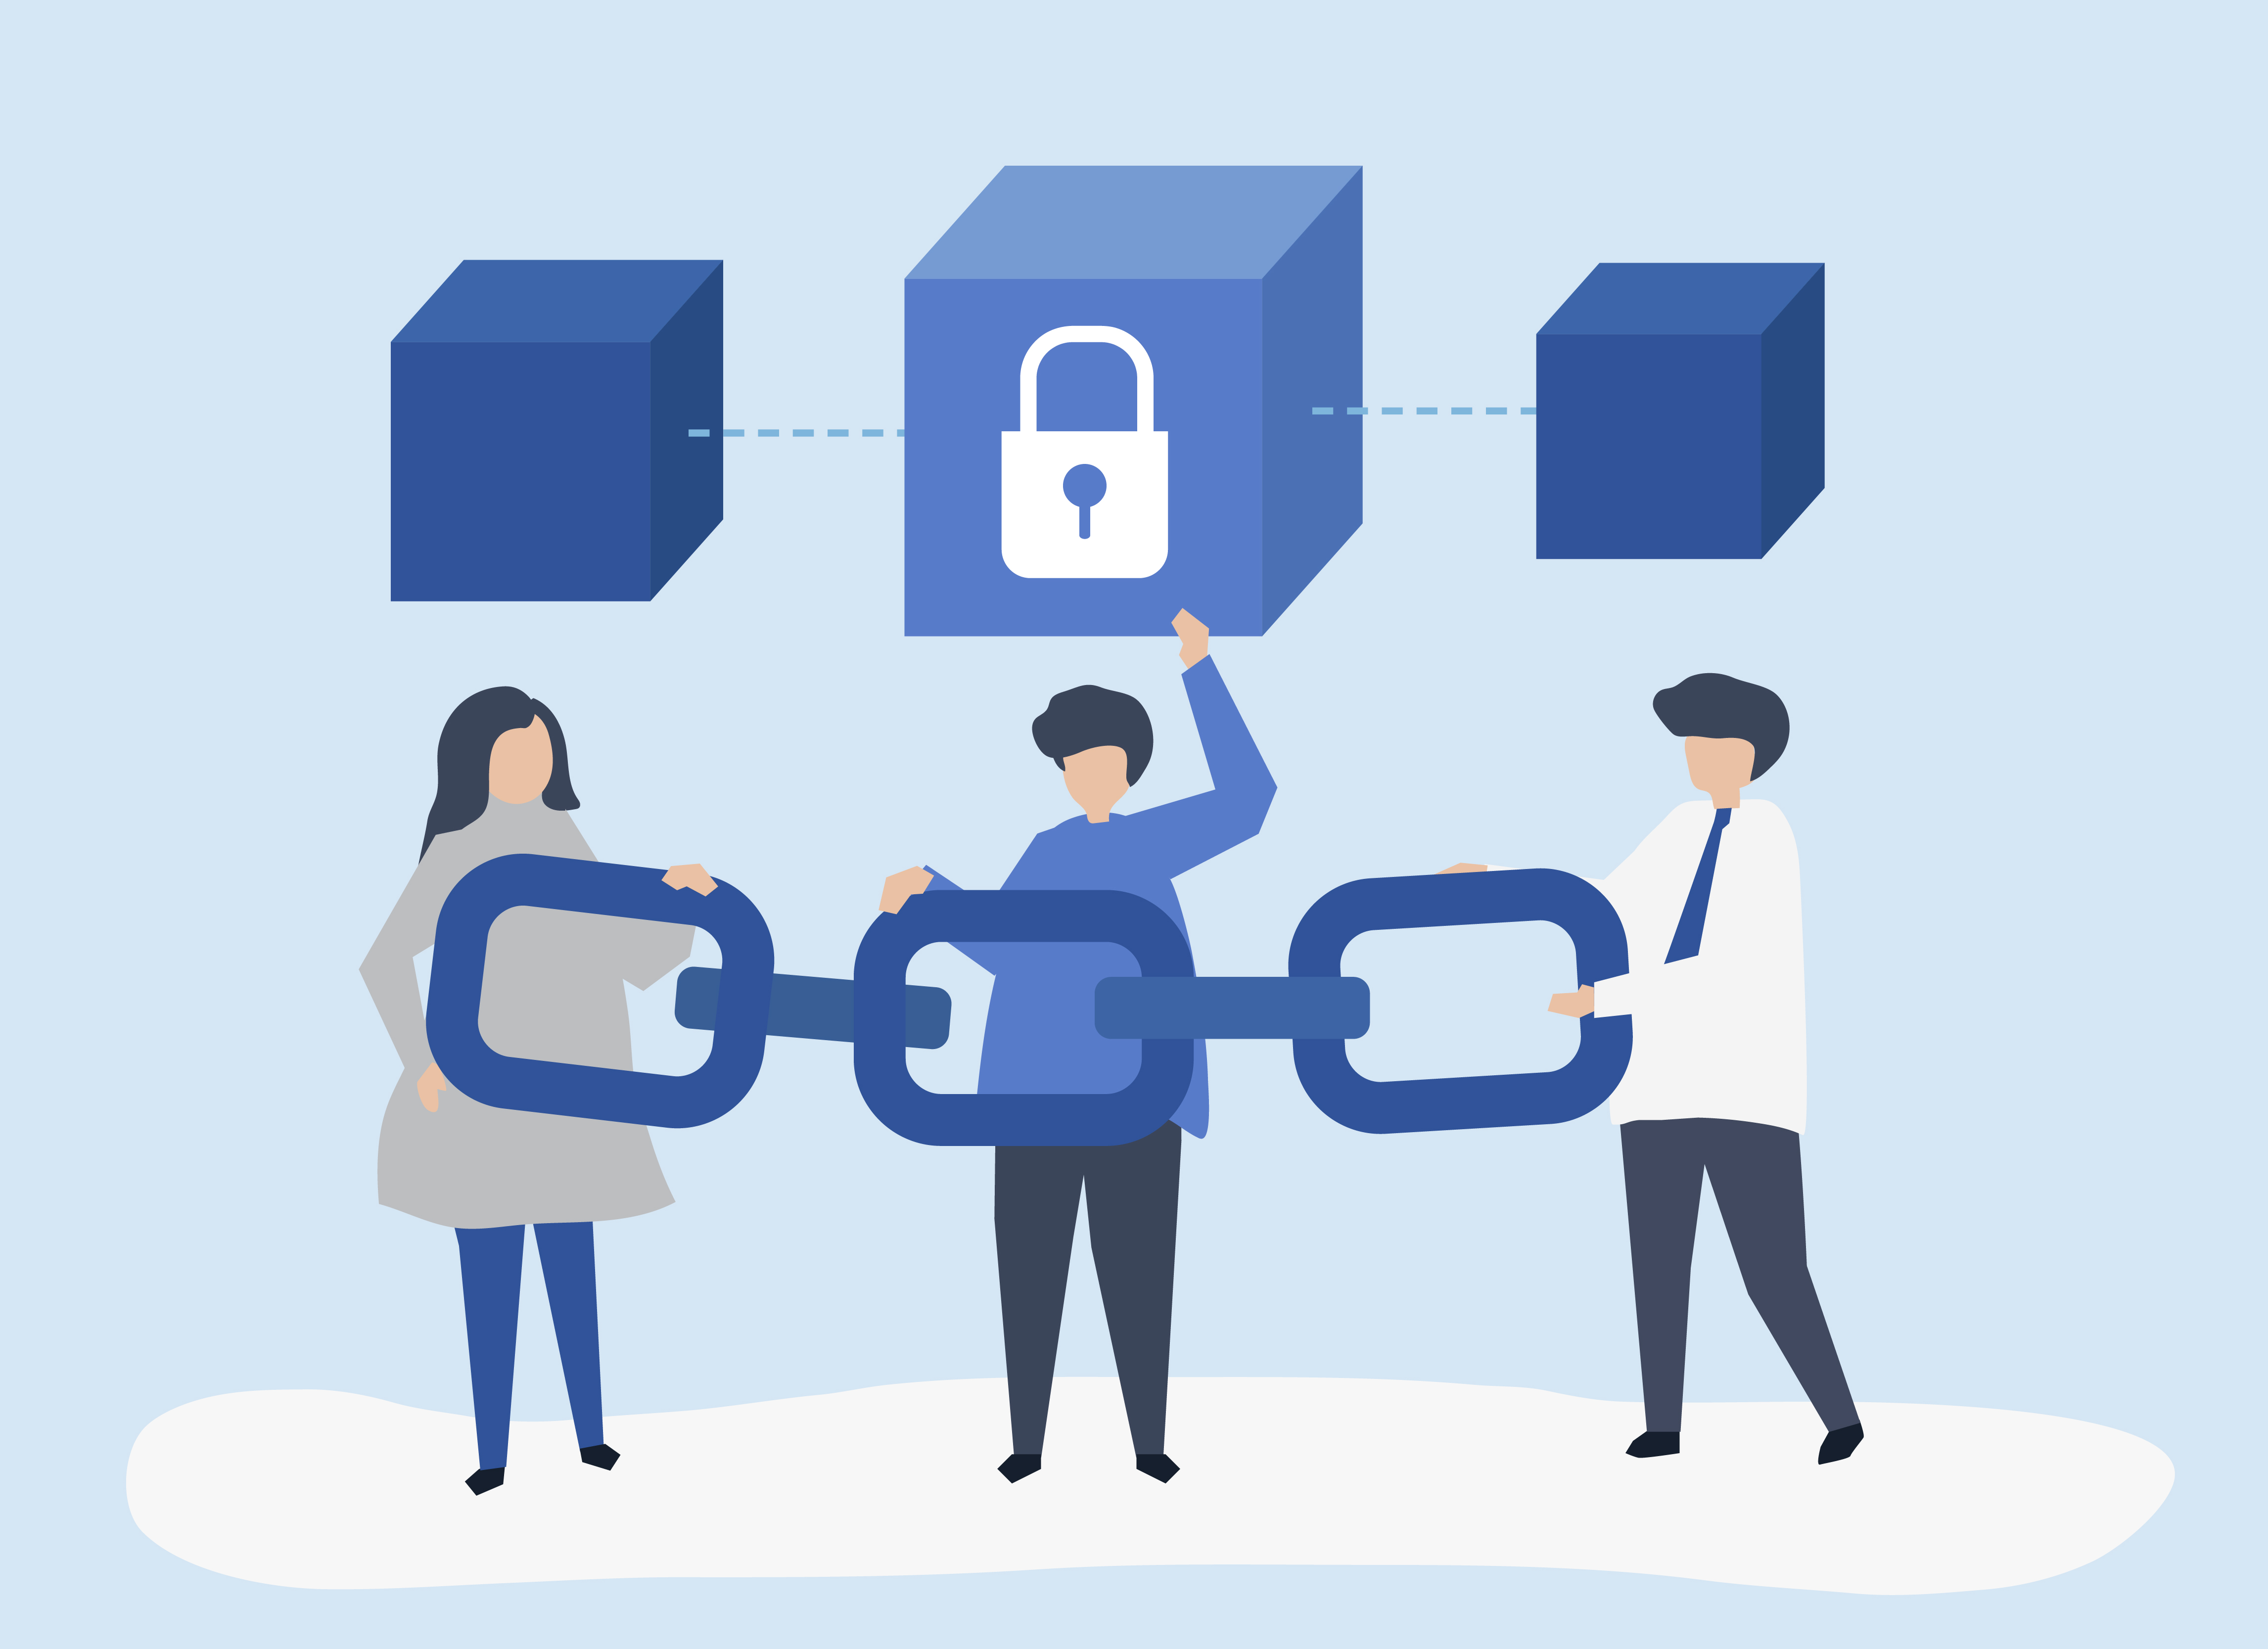
\includegraphics[scale=0.2]{gambar/blockchain-illustrated.jpg}
  \caption{Ilustrasi \emph{Blockchain}}
  \label{fig:blockchainillustrated}
\end{figure}

Untuk dapat dikatakan sebuah \emph{blockchain}, sebuah sistem harus memenuhi beberapa syarat yang dapat ditemui hanya di \emph{blockchain}. Syarat tersebut adalah :

\begin{itemize}
\item{\emph{Immutability}}\\Adalah suatu syarat bahwa data apapun yang telah termuat di dalam suatu blok harus tidak bisa diubah oleh siapapun dalam blockchain tersebut. Yang dimaksud di sini adalah sistem tersebut mempunyai segelintir aturan yang ditetapkan agar data yang telah termuat di suatu blok tidak diubah semena-mena.
\item{Terdistribusi}\\Data yang ada dalam blokchain harus didistribusikan ke seluruh pengguna yang terhubung baik melalui node maupun melalui langsung. Blok data yang terdistribusi harus dimiliki oleh semua penggna.
\item{Tranparan}\\Data yang dikirim pun tidak boleh melalui proses selektif sistem. Blok data yang dikirim oleh blockchain harus seadanya dan tanpa ada modifikasi.
\item{Terdesentralisasi}\\Terdesentralisasi artinya tidak ada pihak utama dalam suatu blockchain yang mengambil keputusan blockchain tersebut. Alih - alih node yang telah terhubung harus membiarkan hal ini tetap terjadi.
\item{Aman}\\Tentu untuk menjamin \emph{Immutability} diperlukan pengamanan yang tepat untuk menjalankan blockchain secara paralel dan tidak terinterupsi.
\item{Konsensus}\\Konsensus adalah sebuah mekanisme kesepakatan yang digunakan oleh blockchain untuk menjaga seluruh sistem tetap adil untuk semua orang. Tentu konsensus ini juga diperlukan agar sistem bisa berjalan cepat dan efektif dalam membuat blok baru.
\end{itemize}

\emph{Blockchain} memiliki banyak konfigurasi mulai dari jenis kriptografi yang digunakan, konsensus yang digunakan, hingga pengaplikasian yang digunakan. Salah satu pembeda \emph{Blockchain} yang cukup terlihat adalah jenis konsensus yang digunakan. Konsensus adalah proses pemufakatan yang dilakukan oleh pengguna dalam suatu jaringan \emph{Blockchain}. Saat ini banyak jenis konsesus yang digunakan mulai dari \emph{Proof of Work, Proof of Authority}, hingga \emph{Proof of Stake}. Dalam sistem sebuah Blockchain terdapat berbagai konfigurasi yang digunakan. Berfokus pada fitur dan keunggulan masing masing. Konfigurasi tersebut berupa jenis konsensus yang dipakai, enkripsi yang digunakan, smart contract yang bisa digunakan, hingga dokumentasi untuk forking blockchain tersebut.
\\ \\ \\
Dalam susunan suatu blok dari blockhain terdapat standar isi dari suatu blok yang telah terbuat. Dalam satu blok yang telah terbuat, terdapat block header, signature, isi transaksi, dan kunci publik. Dalam blok tersebut signature diidentifikasikan sebagai tanda seseorang melakukan transaksi. Tanda tersebut unik dan tidak bisa sama dengan satu yang lain. Juga dalam blok ada kunci publik yang didapatkan dari hash function dalam proses enkripsi pesannya. Kemudian dalam block header teradapat beberapa sub bagian yang berisi mulai dari hash saat ini dan hash sebelumnya, waktu pembuatan blok, dan nonce (numbers only used once) atau nomor tambahan hash yang menandakan kesulitan dari pembuatan blok tersebut. Berikut ilustrasi dari susunan blok dari blockchain.

\begin{figure}[htp]
  \centering
  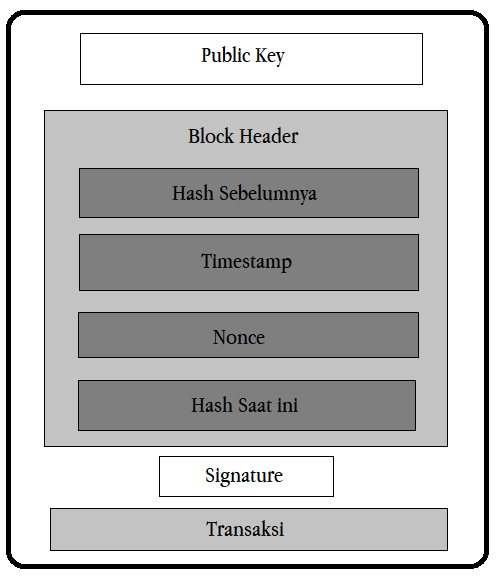
\includegraphics[scale=0.6]{gambar/isi-blok.png}
  \caption{Ilustrasi isi blok}
  \label{fig:isiblok}
\end{figure}

Dari blok yang dibuat, dapat dilihat dari ilustrasi gambar di atas ada beberapa bagian dari suatu blok.Ilustrasi ini merupakan ilustrasi penyederhanaan isi dari suatu blok dari Ethereum. Dalam suatu blok terkandung beberapa bagian yaitu public key, block header, transaksi, dan digital signature. Public key adalah sebuah serangkaian hash yang digunakan sebagai autentikasi data dari transaksi Ethereum. Kemudian ada block header sebagai inti dari sebuah blok dari blockchain yang berisi hash saat ini, kapan transaksi dilakukan dan durasi transaksi, hash sebelumnya, nonce, hingga jenis transaksi yang dilakukan. Semua dapat terlihat pada gambar berikut.

\begin{figure}[htp]
\centering
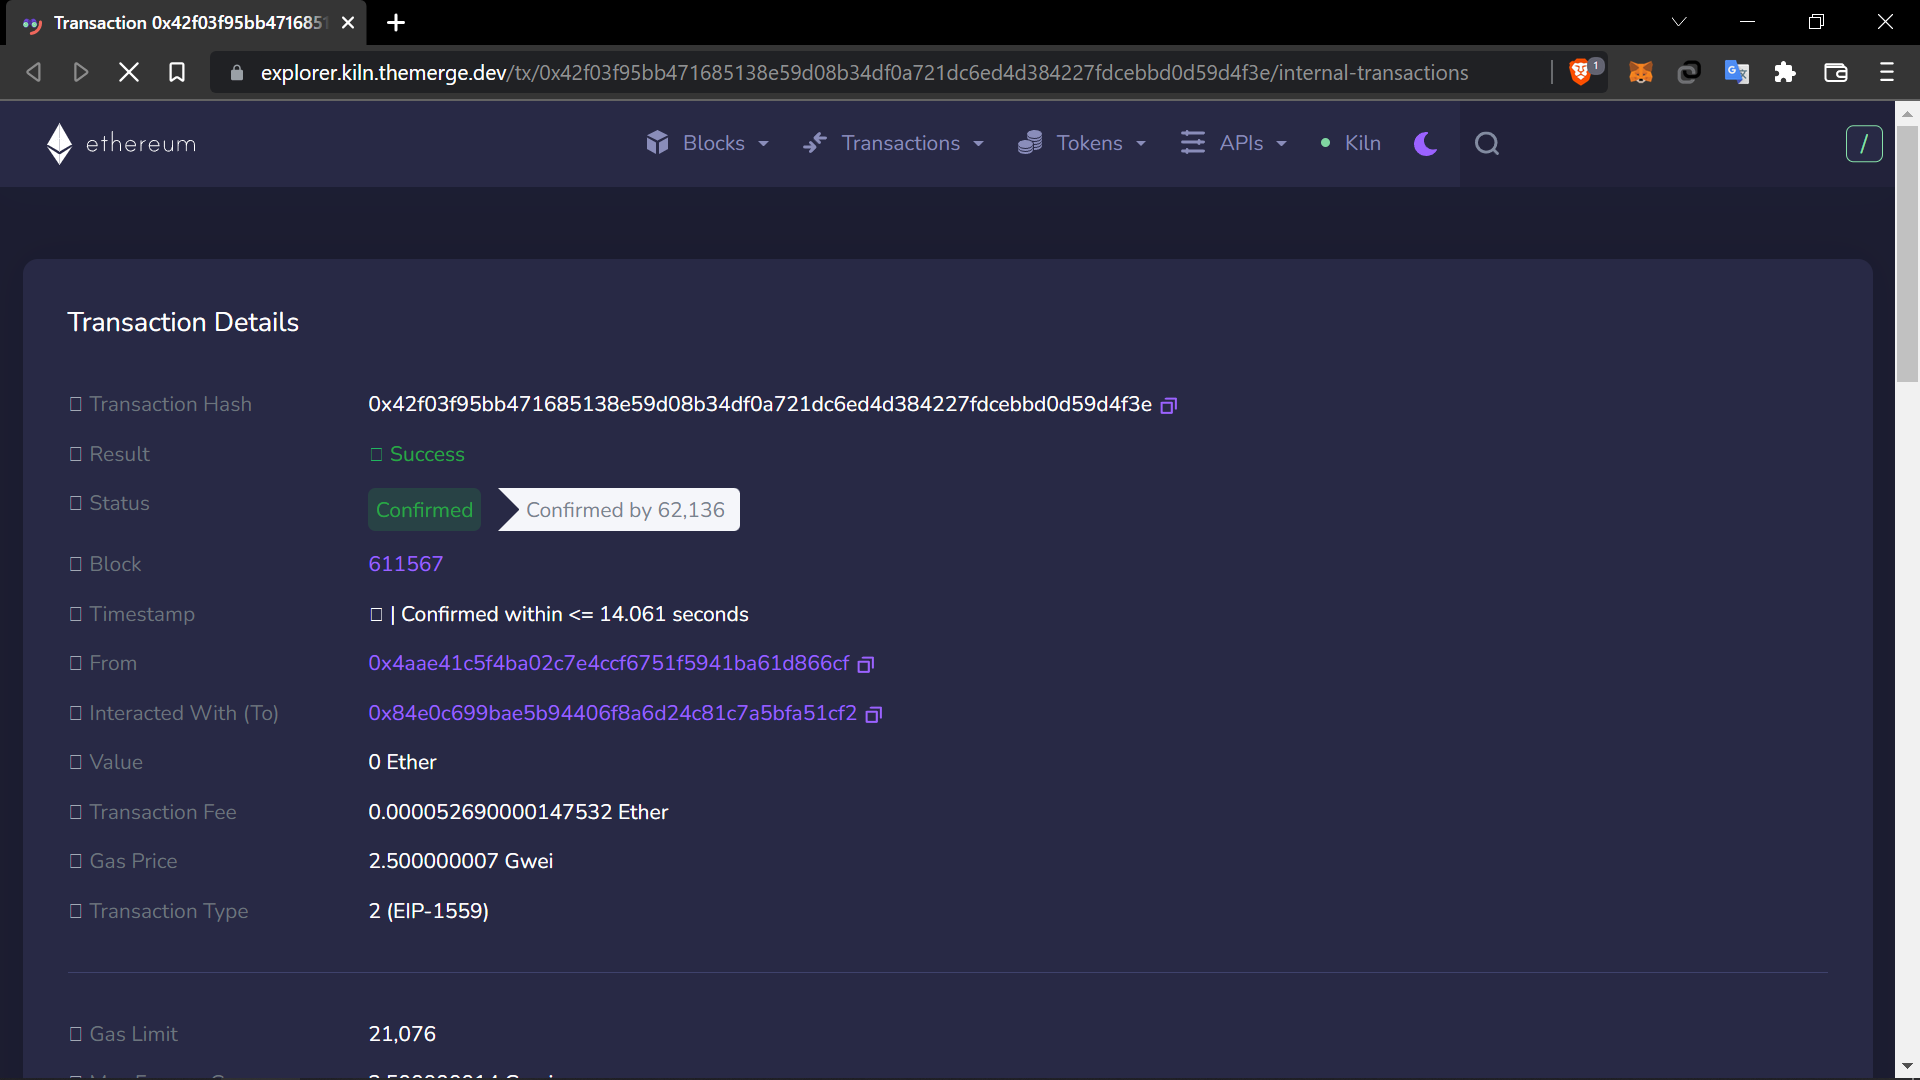
\includegraphics[scale=0.2]{gambar/isi-blok-2.png}
\caption{Gambar isi suatu blok dari blockchain} 
\label{fig:isiblok2}
\end{figure}

Kemudian, dalam blok juga terdapat signature yang dilakukan. Signature ini adalah sebagaian hash yang ditambahkan di dalam hash saat ini yang menandakan jenis yang memvalidasi transaksi yang dilakukan. Seperti pada contoh gambar dibawah terdapat Hex 0x2000 yang merupakan tanda transaksi dilakukan dari Smart Contract yang dibuat. Terakhir, transaksi yang telah dilakukan perincian jumlah gas yang dipakai, harga gas, nonce, hingga harga yang dibayarkan. Berikut isi dalam blok Ethereum.

\begin{figure}[htp]
\centering
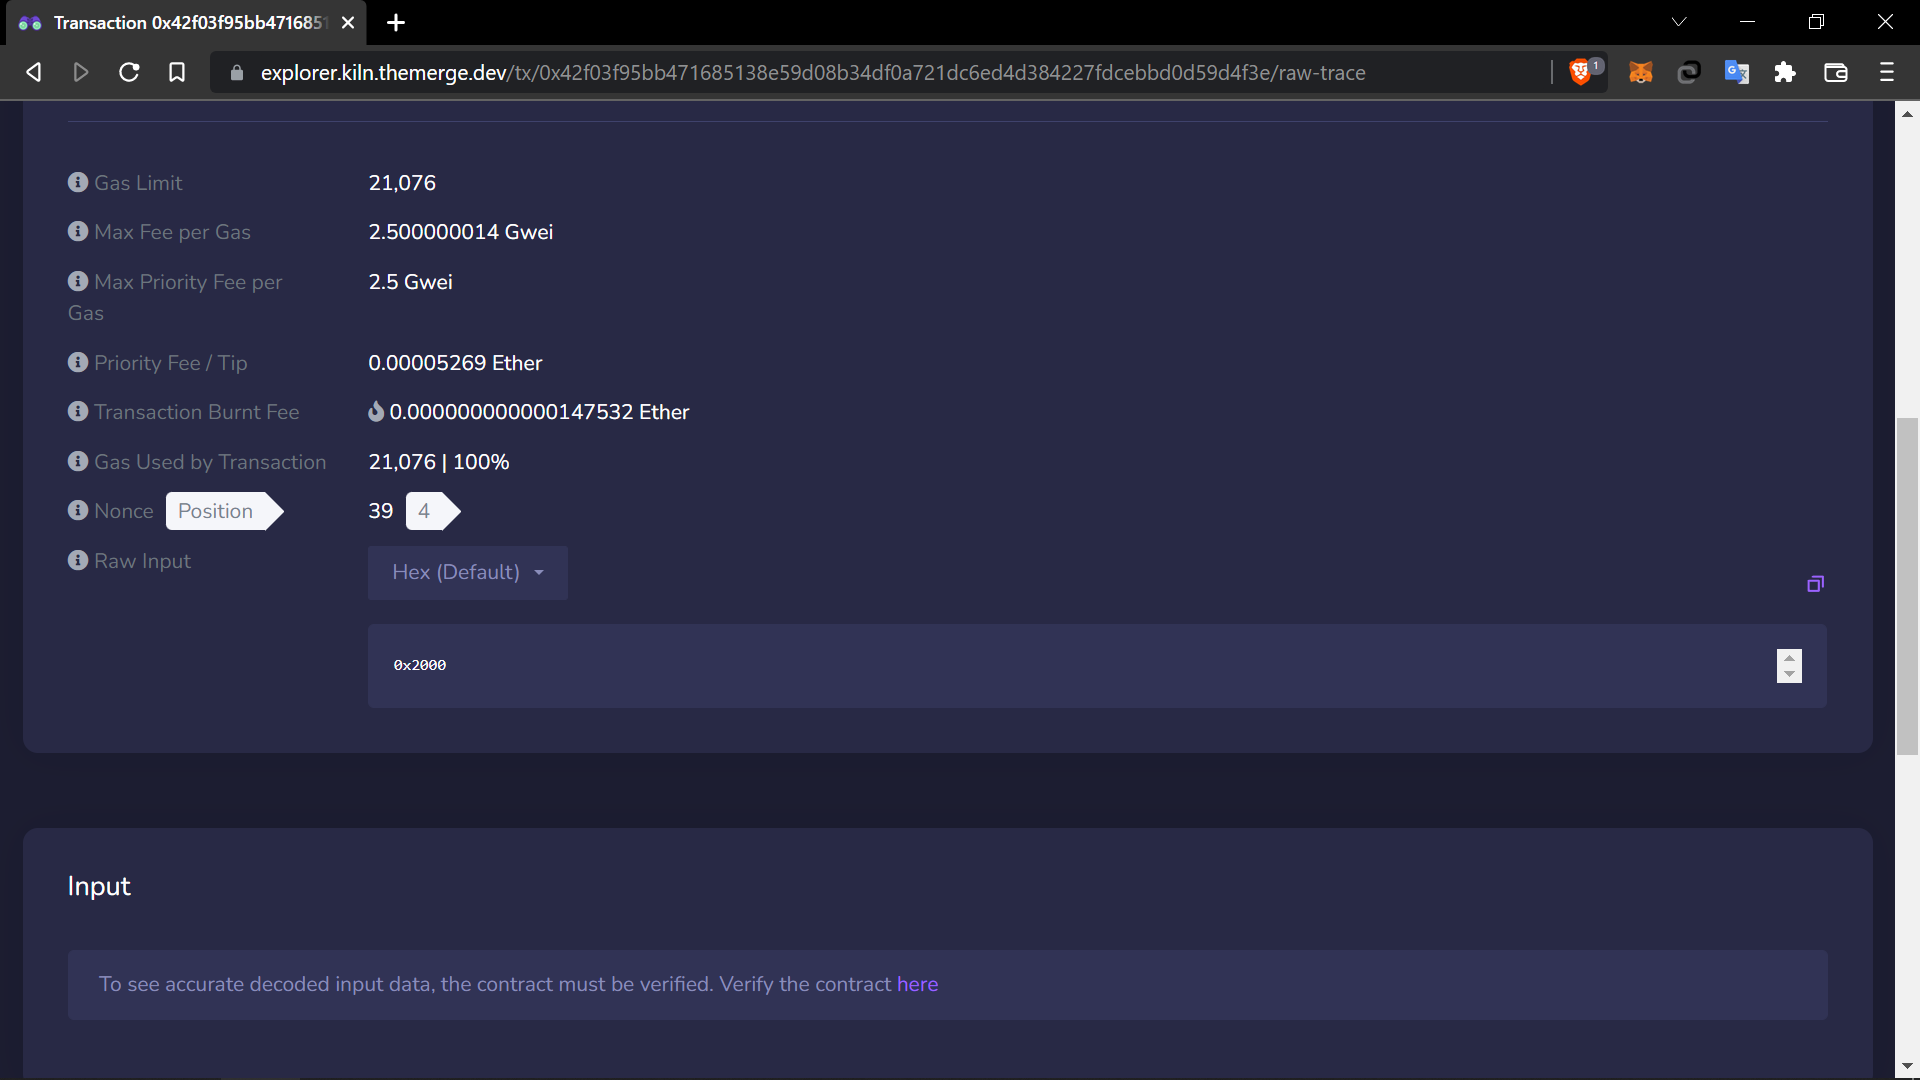
\includegraphics[scale=0.2]{gambar/isi-blok-3.png}
\caption{Isi dari Blok}
\label{fig:isiblok3}
\end{figure}

\subsection{Decentralized Applications}
\label{subsec:dapps}

\begin{figure}[htp!]
\centering
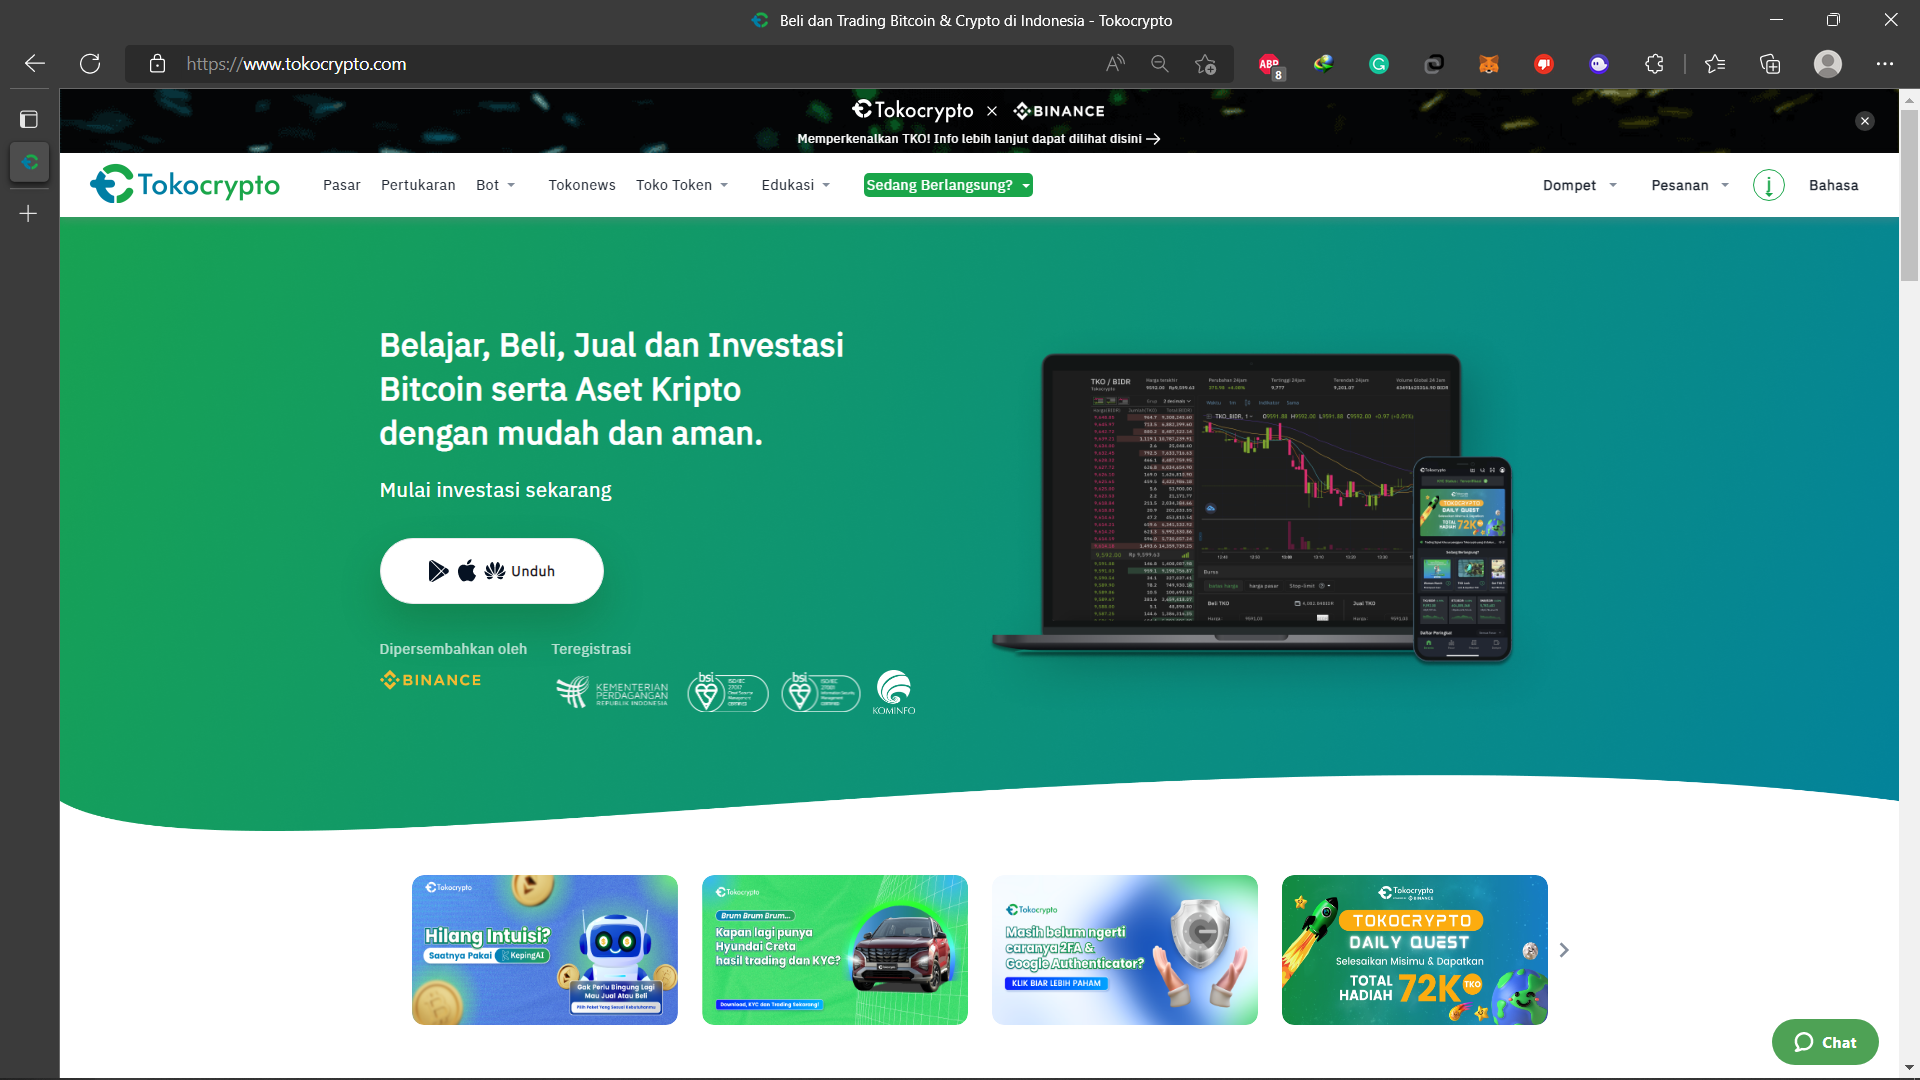
\includegraphics[scale=0.2]{gambar/tokocrypto.png}
\caption{Contoh salah satu Decentralized App di Indonesia, yaitu Tokocrypto : Exchanger Crypto di Indonesia}
\label{fig:tokocrypto}
\end{figure}

Decentralized applications adalah sebuah konsep aplikasi berbasis yang terintegrasi dengan blockchain. Decentralized ini adalah sebuah peleburan antara web 2.0 dengan web 3.0. Peleburan aplikasi ini dimaksudkan sebagai aplikasi yang bisa menyokong Decentralized app ini terdiri atas beberapa bagian yaitu backend, frontend, data storage, hingga protokol komunikasi \cite{MasteringEthGavinWood}. Untuk bisa disebut sebagai decentralized apps, sebuah aplikasi harus memenuhi ketiga aspek:

\begin{itemize}
\item{Ketahanan}
\\ Ketahanan dalam mengelola pelbagai transaksi dalam satu waktu, maka dari itu decentralized apps perlu kemampuan bertahan dalam kondisi menjalankan pelbagai transaksi meski dengan perawatan sistem yang tidak menentu.
\item{Transparan}
\\ Dalam keadaan default, suatu blockchain harus memberikan transparansi kepada seluruh penggunanya. Segala seluk beluk aplikasi mulai dari source code, kerjasama,hingga segala persetujuan bisa dilihat dan diaudit oleh semua pengguna. Dan segala bentuk perubahan harus disimpan di blockchain itu sendiri.
\item{Censorship Resistance}
\\ Pengguna harus mampu mengoperasikan decentralized app dalam secara langsung tanpa ada tokoh penengan tersentral. Artinya dalam pengoperasiannya pengguna harus mampu mengakses decentralized app melalui suatu node dengan mudah.
\end{itemize}

\subsection{\emph{Proof of Stake}}
\label{subsec:pos}

\emph{Proof of Stake} atau PoS adalah sebuah konsensus yang mengambil keputusan berdasarkan sejumlah pertaruhan sebuah pengguna yang terdaftar di dalam jaringan \emph{Blockchain}. Dalam praktiknya PoS tidak memanfaatkan kemampuan komputer pengguna yang terhubung dengan jaringan melainkan memanfaatkan seberapa banyak \emph{cryptocurrencies} yang dia miliki di dalam jaringan tersebut. Banyaknya \emph{cryptocurrencies} yang pengguna miliki akan memengaruhi proses konsensus yang terjadi di jaringan tersebut dan meningkatkan probabilitas pengguna tersebut untuk dipilih untuk berpartisipasi untuk membuat blok dari rangkaian blok yang sedang dibuat \cite{poscons}. Diatas kertas PoS memiliki beberapa keunggulan tersendiri. Dikarenakan tidak menggunakan komputer yang pengguna gunakan, maka PoS tidak memerlukan energi yang besar untuk menjalankan proses pembuatan blok. Kemudian dikarenakan tidak menggunakan energi yang besar otomatis waktu yang dibutuhkan untuk melakukan pembuatan blok pun tidak membutuhkan waktu banyak. Serangkaian kegiatan yang dilakukan oleh PoW seperti memecahkan kriptografi tidak perlu dilakukan dengan waktu yang lama. PoS banyak digunakan di beberapa \emph{blockchain} yang ada seperti Cardano, Solana, hingga Ethereum 2.0.
\\
\emph{Proof of Stake} sendiri dikarenakan menggantikan sebuah konsesus yang telah ada ditargetkan PoS akan memiliki implementasi yang lebih baik dari PoW. Pertama bisa digunakan dalam perangkat \emph{low-power} yang biasa ditemui di masyarakat seperti IoT. Terlebih PoS akan meningkatkan kesempatan perangkat yang terhubung untuk berinteraksi tanpa konsumsi energi yang tinggi. \emph{Proof of Stake} juga mempunyai keunggulan yang tidak dimiliki \emph{Proof of Work} yaitu kemudahan. Tentu kemudahan yang dimaksud yaitu kemudahan dalam setup dan validasi menggunakan perangkat di jaringan \emph{Blockchain} berbasis \emph{Proof of Stake}. Dengan menggunakan \emph{Proof of Stake} pengguna maupun validator tidak memerlukan banyak bahan untuk melakukan persiapan dan ikut dalam jaringan ini. 

\section{\emph{Ethereum}}
\label{sec:eth}

\emph{Ethereum} adalah sebuah blockchain yang menggunakan konsendus \emph{Proof of Stake} untuk membuat blok. Pada sistem Ethereum, sistem ini bersifat open-source dan terdesentralisasi. Dibuat pertama kali pada tahun 2013 oleh Vitalik Buterin, awalnya dibuat sebagai sistem mesin berbasis transaksi yang mana dalam inisiasi sistem terdapat blok pertama dari sebuah blockchain yang berisi instruksi awal dari seluruh sistem mulai dari konsensus, cara pembuatan blok, limit gas, harga gas, hingga alamat awal (yang biasa disebut sebagai blok genesis) kemudian blok utama ini melakukan segala perintah dari blok genesis kemudian melakukannya berulang kali di seluruh mesin yang terhubung ke dalam sistem ini \cite{MasteringEthGavinWood}. Ethereum dibuat sebagai kompetitor dari Bitcoin yang telah diluncurkan dari tahun 2009 bukan hanya sekedar pengganti uang fisik, namun sebagai sebuah sistem terorganisir yang bisa saling berinteraksi dan beririsan antara satu bisnis dengan bisnis lainnya. Ethereum sebagai blockchain yang bersaing langsung dengan Bitcoin sendiri punya beberapa keunggulan dibandingkan dengan Bitcoin. Berikut adalah perbedaan Ethereum dengan Bitcoin secara umum:

\begin{longtable}{|p{4cm}|p{5cm}|p{5cm}|}
  \caption{Tabel Perbandingan \emph{Ethereum} dan \emph{Bitcoin} sebagai sistem Blockchain}
  \label{tb:ethvsbitcoin}\\
  \hline
  \rowcolor[HTML]{C0C0C0}
  \textbf{Aspek} & \textbf{Ethereum} & \textbf{Bitcoin} \\
  \hline
Tahun Peluncuran & 2009 & 2015 \\
  \hline
Konsensus yang digunakan & Proof of Work dan Proof of Stake & Proof of Stake \\
  \hline
Waktu pembuatan blok & ~10 menit & 10-15 detik \\
  \hline
Jumlah suplai & 21 juta & tidak terbatas \\
  \hline
Perkiraan kemampuan transaksi per detik & 7 & 30 \\
 \hline
\end{longtable}

Pada awal perilisan,Ethereum menggunakan PoW untuk melakukan segala proses pembuatan blok dan \emph{scalability}. Karena hal tersebut pada perkembangan awal jaringan ini sangat memerlukan komputer yang mampu untuk melakukan segala proses yang terjadi. Mulai dari memilik pengguna, membuat blok, hingga pengiriman blok memerlukan komputer yang mampu. Dalam satu sisi PoW ini bermanfaat karena pada awal jaringan memerlukan konsensus yang sederhana tidak memerlukan banyak pemrograman. Selain itu PoW juga membuat sistem objektif dalam memilih pengguna untuk membuat blok. Kemungkinan untuk didominasi lebih kecil karena apabila akan melakukan dominasi, perlu banyak hardware yang dikorbankan dan energi yang dikonsumsi sangat besar bahkan memerlukan jaringan energi khusus \cite{poscons}. Karena hal ini Ethereum melakukan proses migrasi menuju konsensus yang lebih hemat energi yaitu PoS. PoS bermaksud untuk mengurangi konsumsi energi secara derastis dan meningkatkan \emph{scalability} yang lebih baik.

\subsection{Ethereum Virtual Machine}
\label{subsec:evm}

Ethereum Virtual Machine adalah sebuah bagian dari Ethereum yang merupakan tempat melakukan interaksi dan deploy Smart Contract \cite{MasteringEthGavinWood}. EVM adalah komputer tempat melakukan berbagai kegiatan dan pelaksanaan transaksi Smart Contract. EVM pada sistem Etherum sendiri merupakan tempat eksekusi program berbahasa Solidity. EVM dapat memilah apa saja yang bisa dilakukan dengan EVM dan apa saja yang tidak bisa dilakukan dengan EVM. EVM mempunyai arsitektur seperti berikut :
\\
\begin{figure}[htp]
\centering
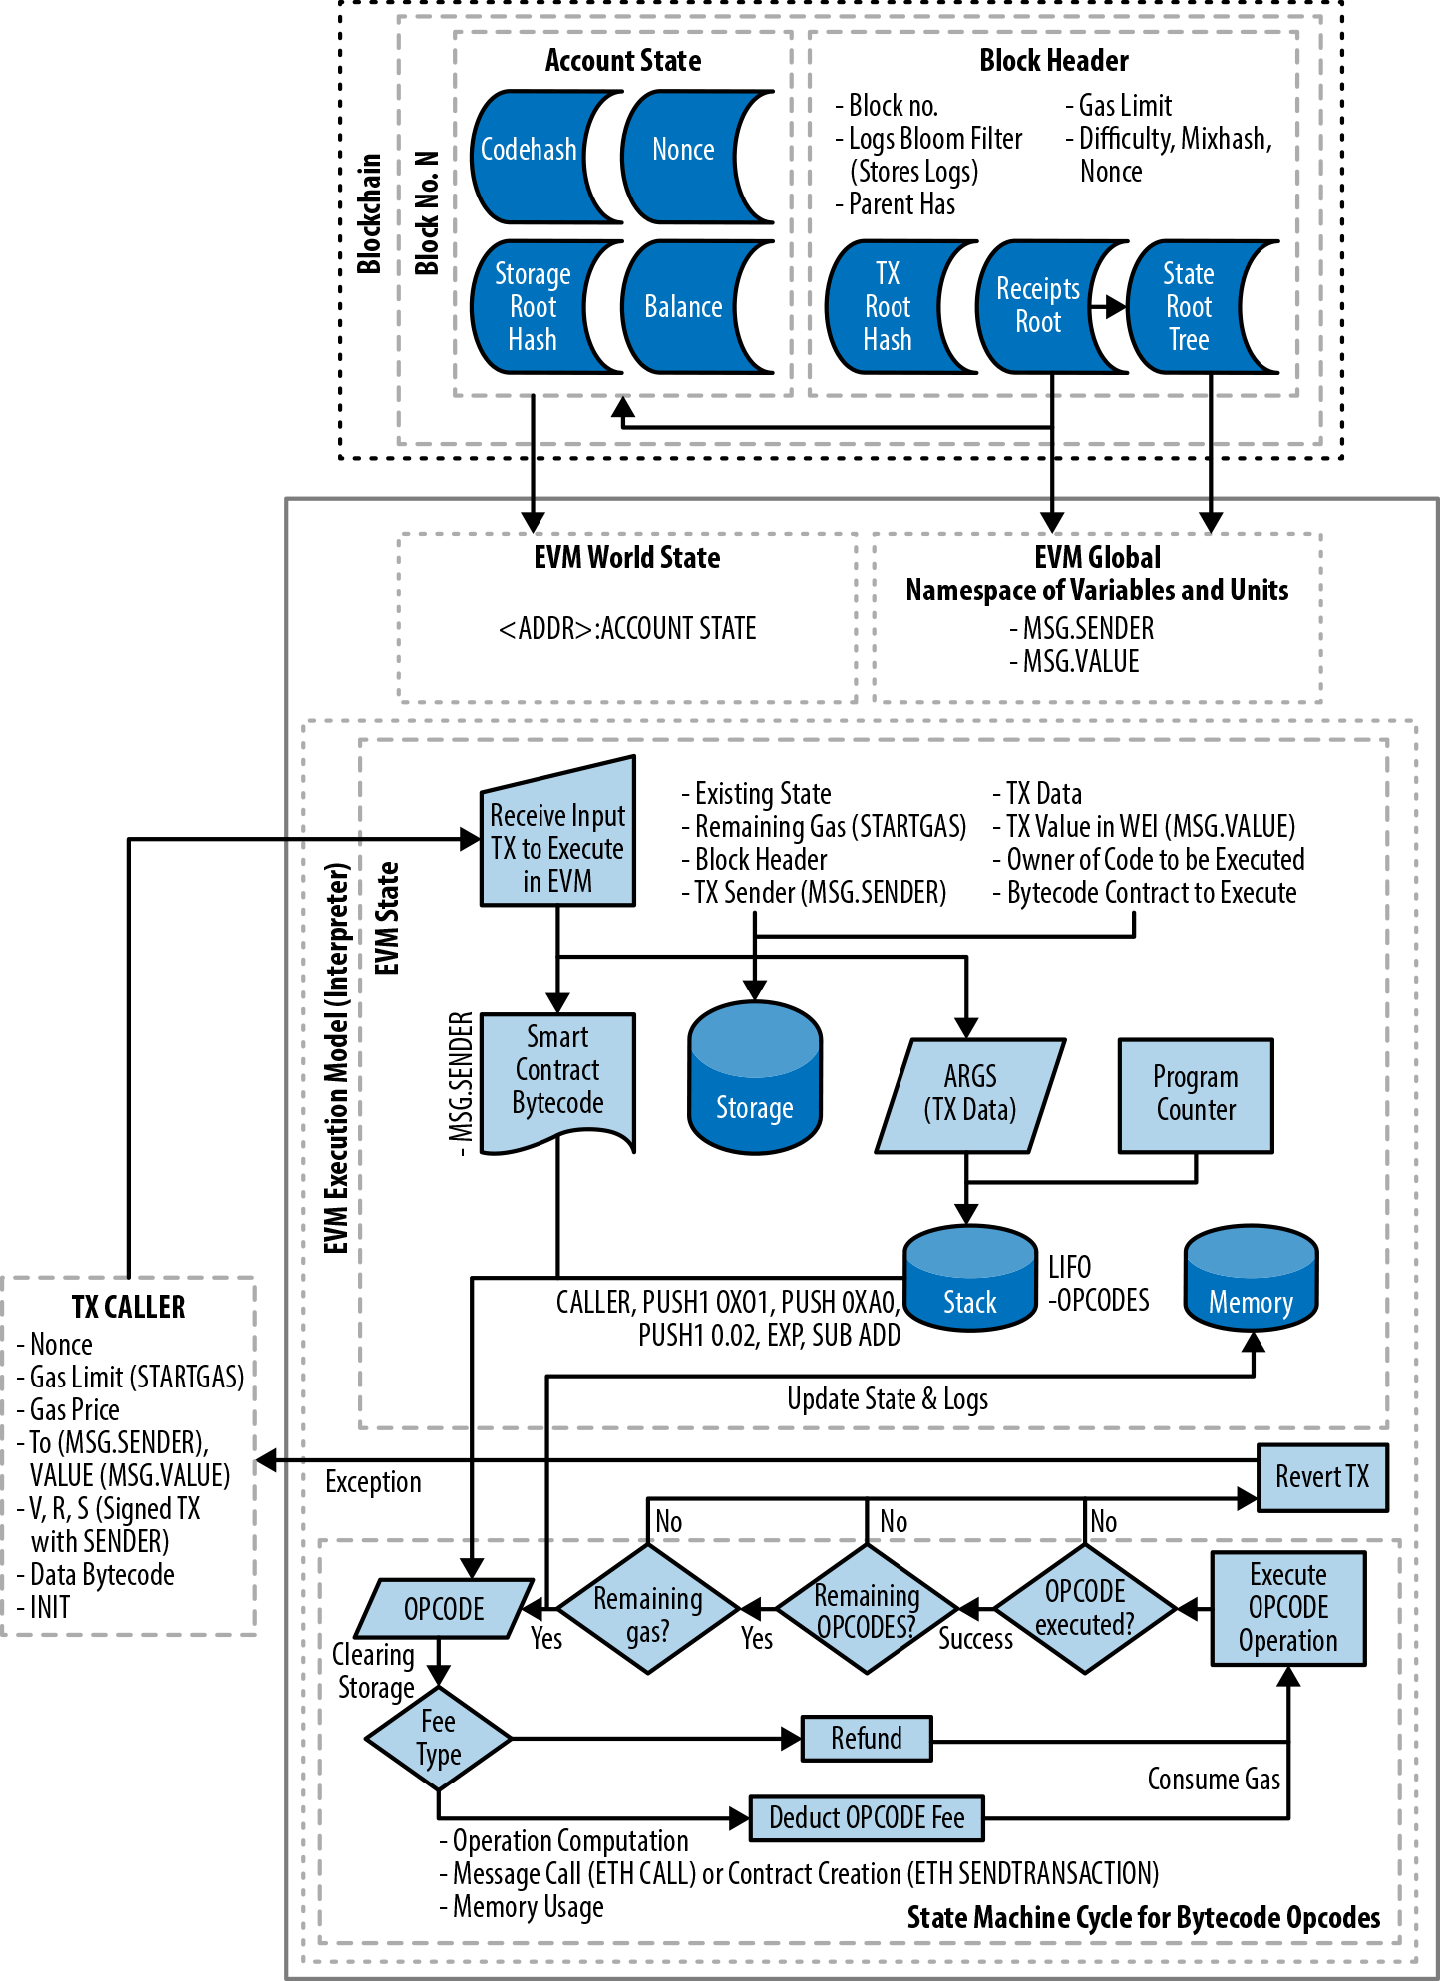
\includegraphics[scale=1.2]{gambar/arsitektur-evm.png}
\caption{Arsitektur EVM}
\end{figure}

Pada gambar arsitektur, dapat dilihat EVM memilah dan menjalankan program sesuai dengan ketersediaan gas yang diberikan dari akun yang melakukan request transaksi. Seperti yang telah dijelaskan pada 2.4.1, gas diperlukan sebagai biaya utama untuk diberikan ke pada EVM untuk melakukan proses deploy dan interaksi Smart Contract. Gas ini digunakan di dalam EVM untuk mengeksekusi program dengan harga variatif. Berikut harga untuk beberapa operasi aritmatika maupun kompleks:
\begin{itemize}
\item{Penambahan dan Pengurangan}\\Untuk operasi ini bernilai 3 gas unit
\item{Perkalian dan Pembagian}\\Untuk operasi ini bernilai 5 gas unit
\item{Logic operation}\\Untuk operasi ini bernilai 3 gas unit
\item{Hashing}\\Untuk operasi SHA3 hash bernilai (30 + 6*(\emph{n})) gas unit dengan \emph{n} untuk setiap 256 bit data yang telah melalui operasi hash
\item{Mengirim transaksi}\\Untuk mengirimkan transaksi bernilai 21000 gas unit
\item{Mengecek saldo}\\Untuk mengecek saldo bernilai 400 gas unit
\item{Info umum}\\Untuk mengecek address, caller, dan timestamp bernilai 2 gas unit
\item{Membuat blok}\\Untuk membuat blok bernilai 32000 gas unit
\item{Memanggil fungsi}\\Untuk memanggil fungsi bernilai mulai dari 700 gas unit
\item{Pembukaan akun}\\Untuk membuat akun diperlukan bernilai 30000 gas unit dan untuk menghapus atau mengedit akun bernilai 5000 gas unit 
\end{itemize}
Karena EVM melakukan perhitungan sebagai \emph{stack machine} dengan nilai satu blok memori sebesar 256 bit. EVM mempunyai beberapa instruksi set yaitu:
\begin{itemize}
\item{Aritmatika dan Logic Operations}
\item{Logging}
\item{Control Flow}
\item{Stack, Memory, dan akses penyimpanan}
\item{Pencarian kode}
\end{itemize}

\subsection{Perbedaan \emph{Proof of Stake} dan \emph{Proof of Work}}
\label{subsec:powandposdiffer}

Dalam proses seleksi siapa yang berhak untuk menjadi validator dalam suatu transaksi \emph{Ethereum}, terdapat beberapa kesepakatan bersama/konsensus yang digunakan dalam memilih validator. Saat ini terdapat dua konsensus yang umum digunakan berbagai macam \emph{Cryptocurrencies} yaitu \emph{Proof of Stake} dan \emph{Proof of Work} \cite{9388487}. Berikut adalah perbandingan antara keduanya.

\begin{longtable}{|p{4cm}|p{5cm}|p{5cm}|}
  \caption{Tabel Perbandingan \emph{Proof of Stake} dan \emph{Proof of Work}}
  \label{tb:posandpowdifference}\\
  \hline
  \rowcolor[HTML]{C0C0C0}
  \textbf{Ciri} & \textbf{Proof of Stake} & \textbf{Proof of Work} \\
  \hline
Cara membuat blok & Melakukan validasi pengirim dan penerima dengan mencocokkan kunci publik antara satu dengan lainnya & Melakukan pemecahan soal matematika kompleks untuk melakukan suatu transaksi \\
  \hline
  Memilih validator & Berdasarkan jumlah \emph{cryptocurrencies} yang dipegang satu akun & Berdasarkan raw power komputer yang dipegang satu akun \\
  \hline
  Konsumsi daya & Rendah karena tidak memerlukan raw power komputer & Tinggi karena memanfaatkan semua raw power yang diberikan \\
 \hline
 Ketahanan sistem & Sistem tidak terlalu baik karena validator stagnan dan mengonsumsi daya tahan penyimpanan lokal & Sistem cukup baik karena validator selalu meningkatkan raw power komputer. Otomatis perangkat diperbarui secara berkala\\
 \hline
Kecepatan pembuatan blok & Lebih cepat karena tidak perlu raw power komputer & Lebih lambat karena perlu raw power komputer\\
\hline
  Skalabilitas & Cukup baik dalam meningkatkan jumlah transaksi dalam satu interval & Cukup baik dalam meningkatkan jumlah transaksi dalam satu interval\\
\hline 
\end{longtable}
  \cleardoublepage

  % Bab 3 desain dan implementasi
  \chapter{METODOLOGI}
\label{chap:metodologi}

Penelitian ini dilaksanakan dilakukan dalam beberapa tahap. Tahapan tersebut meliputi beberapa persiapan peralatan yang digunakan dan alur/desain penelitian secara menyeluruh. Peralatan ini meliputi perangkat keras dan software yang digunakan untuk melakukan pengujian sistem yang telah dibuat. Kemudian untuk desain secara menyeluruh meliputi bagian frontend yaitu website untuk antarmuka pengguna, Metamask sebagai gateway Ethereum, dan Smart Contract yang menggunakan Ethereum. Berikut adalah rinciannya:

\section{Peralatan}
\label{sec:peralatan}

Untuk peralatan diperlukan peralatan yang bisa digunakan sebagai alat percobaan desain sistem sesuai kebutuhan dari dokumentasi \emph{Ethereum}. Penelitian ini peralatan yang telah digunakan yaitu :

\subsection{Perangkat Keras}
\label{subsec:hardware}

Ada beberapa perangkat yang digunakan pada penelitian ini. Perangkat keras yang digunakan adalah perangkat laptop yang mampu menjalankan software maupun melakukan kegiatan membuat, audit, hingga deploy \emph{Smart Contract}. Selain itu perngakat yang digunakan perlu bisa menghubungkan ke jaringan internet. Perangkat yang digunakan adalah jenis laptop yang mempunyai spesifikasi sebagai berikut:

\begin{table}[htp] 
\caption{Perangkat 1}
\centering
\begin{tabular}
{|p{4cm}|p{9cm}|}
\hline
Processor & AMD Ryzen 5 3500U (4 Core/8 Threads) @2.1GHz TDP 35W, FP4 Socket \\ \hline
RAM & DDR4 16 GB (Dual Channel - 2x8 GB) @2400 MHz \\ \hline
Penyimpanan & 1000 GB HDD SATA III + 512 GB SSD NVMe \\ \hline
Kartu Grafis & iGPU Vega 8, 2 GB @1200 MHz \\ \hline
Sistem Operasi & Windows 10 \\ \hline 
\end{tabular}
\end{table}

\begin{table}[htp] 
\caption{Perangkat 2}
\centering
\begin{tabular}
{|p{4cm}|p{9cm}|}
\hline
Processor & AMD Ryzen 5 3500U (4 Core/8 Threads) @2.1GHz TDP 35W, FP4 Socket \\ \hline
RAM & DDR4 16 GB (Dual Channel - 2x8 GB) @2400 MHz \\ \hline
Penyimpanan & 1000 GB HDD SATA III + 512 GB SSD NVMe \\ \hline
Kartu Grafis & iGPU Vega 8, 2 GB @1200 MHz \\ \hline
Sistem Operasi & Windows 10 \\ \hline 
\end{tabular}
\end{table}

\subsection{Software}
\label{subsec:software}

Software yang digunakan adalah segala software yang digunakan untuk pengembangan desain sistem yang telah dibuat. Software tersebut adalah:

\begin{table}[htp] 
\caption{Software yang Digunakan}
\centering
\begin{tabular}
{|p{4cm}|p{6cm}|}
\hline
Text Editor & Visual Studio Code \\ \hline
Web Browser & Microsoft Edge, Mozilla Firefox, Brave Browser \\ \hline
IDE & Remix \\ \hline
\emph{Ethereum Gateway} & Metamask \\ \hline
\end{tabular}
\end{table}



\section{Desain Sistem}
\label{sec:desainsistem}

Sistem yang akan digunakan adalah gabungan dari Smart Contract dan Frontend. Smart Contract sebagai tempat menyediakan fungsi dan menyimpan data transaksi, sedangkan pada bagian Frontend adalah tempat antarmuka pengguna. Berikut adalah alur kerja yang akan dilaksanakan:

\begin{figure}[htp!]
	\centering
	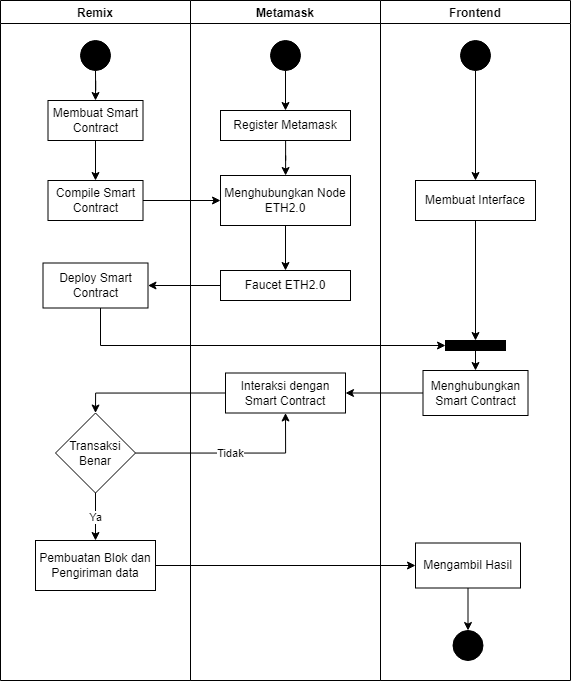
\includegraphics[scale=0.45]{gambar/alur_penelitian.png}
	\caption{Desain sistem penelitan}
	\label{fig:desainsist}
\end{figure}

Untuk desain sistem meliputi dua bagian yaitu \emph{Smart Contract} dan website. Bagian \emph{Smar Contract} memuat fungsi fungsi utama dari dompet yaitu mengirim, menyimpan, dan mengecek. Dan untuk bagian websitenya merupakan antarmuka antara pengguna dengan fungsi dari \emph{Smart Contract}. Berikut adalah penjabaran dari bagian - bagian tersebut:

\subsection{\emph{Smart Contract}}
\label{subsec:smartcontract} 

\emph{Smart Contract} yang digunakan dalam desain sistem ini adalah \emph{Smart Contract} yang menggunakan bahasa Solidity versi 0.6.0 keatas. Untuk Smart Contracnya sendiri memerlukan SPDX License Identifier sebagai syarat yang lebih baik dicantumkan dalam smart contract untuk mencegah hal yang tidak diinginkan. Smart contract ini menggunakan SPDX License MIT.Dalam \emph{Smart Contract} ini berisi beberapa fungsi yaitu:

\begin{lstlisting}[
  language=python,
  caption={Smart Contract Ether Wallet},
  label={lst:smartcontractwallet}
]
//SPDX-License-Identifier:MIT
pragma solidity >=0.8.7;

contract Transactions {

    address payable public owner;

    constructor() {
        owner = payable(msg.sender);
    }

    function deposit() external payable {
    }

    function withdraw() public payable {
        (bool os,)= payable(owner).call{value:address(this).balance}("");
        require(os);
    }

    function withdraw2(uint _amount) external {
        require(msg.sender == owner, "caller is not owner");    
        payable(msg.sender).transfer(_amount);
    }

    function sendEth(address payable receiver, uint _amount) external {
        receiver.transfer(_amount);
    }

    function getBalance() external view returns(uint) {
        return address(this).balance;
    }

    function getAddress() external view returns(address) {
        return address(this);
    }
}
\end{lstlisting}

Dari source code \emph{Smart Contract} tersebut terdapat fungsi lainnya yang ada dalam smart contract ini. Berikut adalah fungsinya :

\begin{enumerate}
\item{\textbf{Konstruktor dan alamat pemilik}}

\begin{lstlisting}[
	language=python,
	caption={Konstruktor dan Alamat Pemilik},
	label={lst:construtorandaddressowner}]

//SPDX-License-Identifier:MIT
pragma solidity >=0.8.7;
//Semua dalam satuan Wei
contract Transactions {
    address payable public owner;

    constructor() {
        owner = payable(msg.sender);
    }
\end{lstlisting}

Pada potongan kode ini, \emph{smart contract} akan menginisiasi siapa pemilik uang dengan mendeteksi \emph{address} dari pemilik dan melakukan construct dari pemilik uang. Semua nominal yang bisa diinteraksikan dengan user menggunakan satuan Wei.

\item{\textbf{Deposit Uang}}
\begin{lstlisting}[
	language=python,
	caption={Fungsi deposit ke Smart Contract},
	label={lst:deposit}]

function deposit() external payable {
    }
\end{lstlisting}
Kedua, pada bagian ini merupakan fungsi untuk mendepositkan sejumlah uang ke dalam Smart Contract.

\item{\textbf{Penarikan Uang}}
\begin{lstlisting}[
	language=python,
	caption={Fungsi penarikan uang dari Smart Contract}
	label={lst:withdraw}]

function withdrawAll() public payable {
        (bool os,)= payable(owner).call{value:address(this).balance}("");
        require(os);
    }

    function withdrawPartial(uint _amount) external {
        require(msg.sender == owner, "Maaf anda bukan Owner");    
        payable(msg.sender).transfer(_amount);
    }
\end{lstlisting}

Ketiga adalah fungsi penarikan uang dari Smart Contract ke alamat pemilik. Ada dua jenis penarikan yang bisa dilakukan yaitu penarikan seluruh uang, atau penarikan parsial.

\item{\textbf{Kirim Uang}}
\begin{lstlisting}[
	language=python,
	caption={Fungsi kirim uang dari Smart Contract ke alamat penerima},
	label={lst:sendEth}]

function sendEth(address payable receiver, uint _amount) external {
        receiver.transfer(_amount);
    }
\end{lstlisting}

Keempat fungsi pengiriman uang ke penerima. Pengiriman ini menggunakan metode transfer dari dokumentasi bahasa pemrograman Solidity. Metode transfer ini digunakan karena bisa melakukan return ketika ada error yang terjadi.

\item{\textbf{Informasi Umum}}
\begin{lstlisting}[
	language=python,
	caption={Fungsi untuk mendapatkan informasi seputar akun dan Smart Contract}
	label={lst:generalinfo}]

function sendEth(address payable receiver, uint _amount) external {
        receiver.transfer(_amount);
    }

    function getBalance() external view returns(uint) {
        return address(this).balance;
    }

    function getAddress() external view returns(address) {
        return address(this);
    }
}

\end{lstlisting}
Terakhir merupakan fungsi untuk mendapatkan informasi alamat pemilik, hash Smart Contract, dan jumlah uang yang tersimpan di Smart Contract.
\end{enumerate}

\section{Alur Pembuatan Sistem}
\label{sec:alurkerja}

Seperti yang telah terlihat dari gambar 3.1: Desain sistem penelitian, akan ada tiga elemen yang perlu dipersiapkan. Berikut adalah penjelasannya:

\subsection{Deploy Smart Contract ke Jaringan ETH2.0}
\label{subsec:how2DeployContract}

Dalam pemrograman Smart Contract pada blockchain Ethereum, tersedia opsi bahasa pemrograman Solidity dengan Remix sebagai IDE. Solidity adalah sebuah bahasa pemrograman yang digunakan untuk membuat suatu \emph{smart contract}. Solidity merupakan bahasa pemrograman berbasis OOP yang terinsipirasi Python, C++, dan JavaScript. Bahasa pemrograman ini merupakan bahasa statis yang diinisiasikan oleh Gavin Wood pada tahun 2014 dan menjadi bahasa pemrograman utama untuk \emph{Ethereum}. Solidity berjalan dan dicompile pada \emph{Ethereum Virtual Machine}. Dan untuk mengoperasikannya memerlukan deklarasi untuk pelbagai variabel,fungsi, hingga memory yang digunakan. Solidity memiliki beberapa fitur pembeda dari bahasa pemrograman lainnya yang serupa seperti struktur database, \emph{inheritance}, \emph{mapping}, hingga multi fungsi dalam satu \emph{smart contract}. Saat ini Solidity telah mencapai versi 0.8.14 dengan memiliki beberapa perubahan pada semantik,penyederhanaan fungsi, hingga perubahan susunan output. Dalam Solidity terdapat kekurangan yaitu ketika smart contract telah dicompile dan dideploy di EVM, maka tidak dapat dilakukan edit pada smart contract tersebut. Karena pembuatan smart contract ini bersifat \emph{irreversible}, maka ketika membuat smart contract perlu dilakukan dengan efektif dan efisien. Untuk mengopersasikan Solidity diperlukan sebuah IDE yang bisa melakukan segalanya. IDE tersebut adalah Remix. Remix adalah IDE online yang terhubung langsung dengan EVM privatnya sendiri. IDE ini memiliki beberapa fitur seperti lokal \emph{Ethereum}, compile, deploy, interaksi dengan smart contract secara langsung, hingga perhitungan harga yang dibayar dan optimalisasi dari smart contract. Remix dapat digunakan secara gratis dan dapat menyimpan data workspace kita ke cloud yang dia miliki. Karena kemudahan ini, Remix banyak digunakan oleh developer Solidity. \\
Untuk bagian deploy Smart Contract ini digunakan.
Selanjutnya akan dijelaskan secara rinci bagaimana deploy Smart Contract ke jaringan ETH2.0.
\begin{enumerate}
\item{Buka Remix di browser, dan buat file .sol baru di folder smart-contract}
	\begin{figure}[htp]
		\centering
		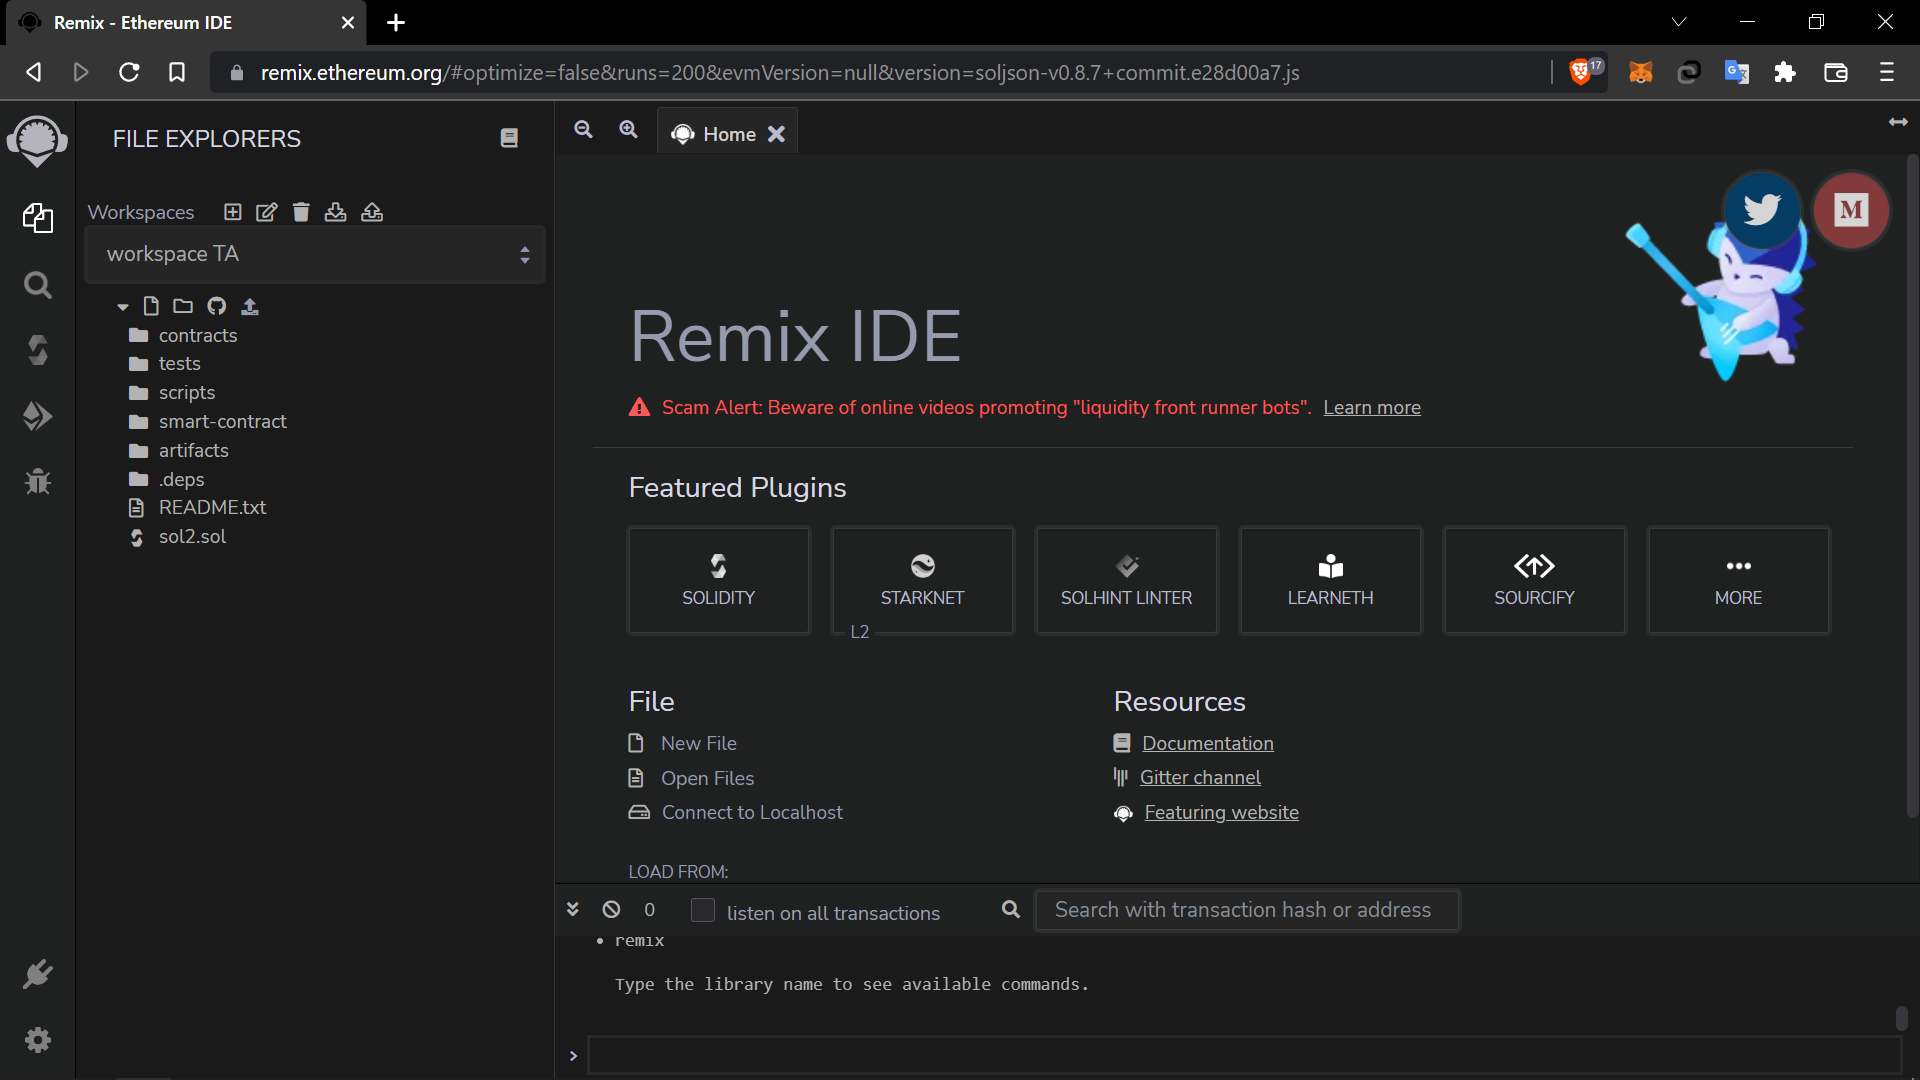
\includegraphics[scale=0.2]{gambar/bab3/deploy/1.png}
		\caption{Tampilan antarmuka Remix IDE}
		\label{fig:guiremix}
	\end{figure}
\item{Masukkan semua source code yang telah dibaut ke dalam .sol file tersebut, kemudian simpan dengan nama sesuai yang diinginkan}
	\begin{figure}[htp]
		\centering
		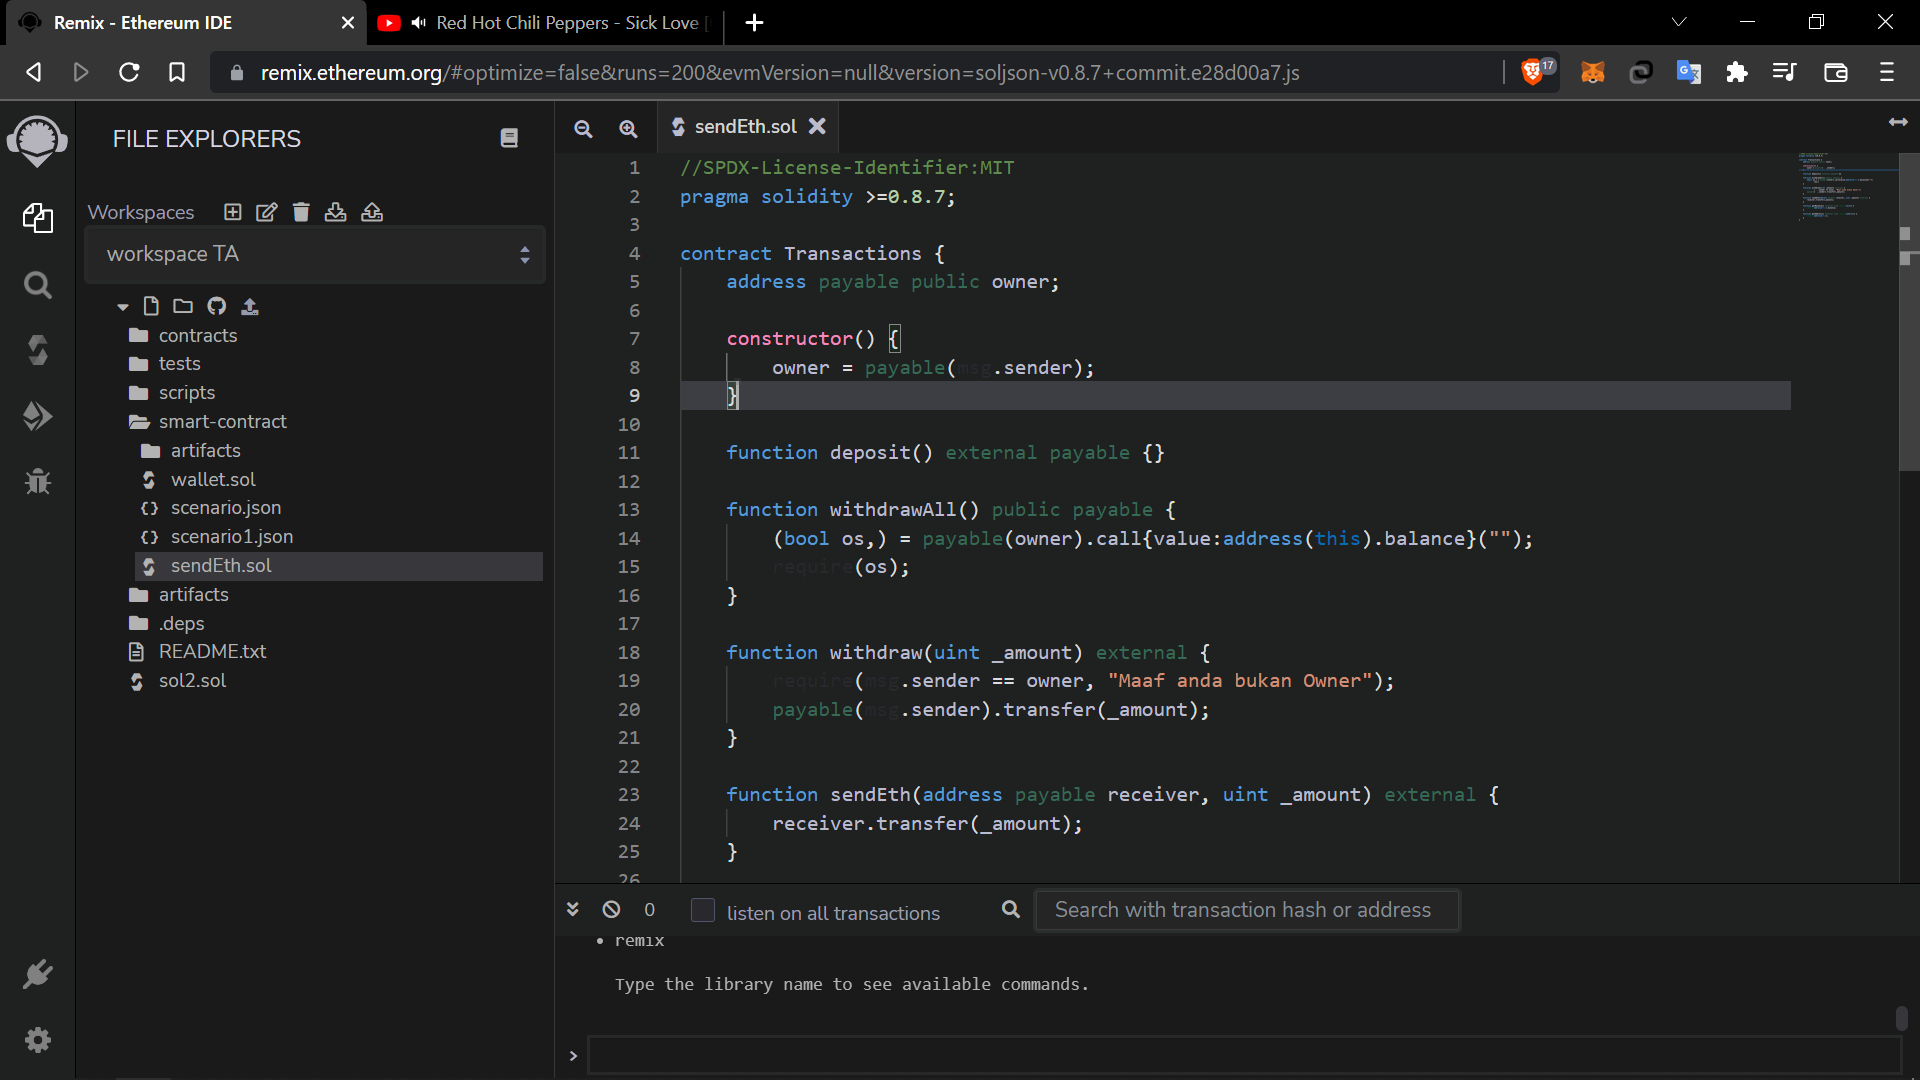
\includegraphics[scale=0.2]{gambar/bab3/deploy/2.png}
		\caption{Memasukkan source code ke dalam file .sol}
		\label{fig:srcsolremix}
	\end{figure}
\newpage
\item{Pada tab bagian kiri, klik Solidity compiler. Kemudian klik Compile file kita}
	\begin{figure}[htp]
		\centering
		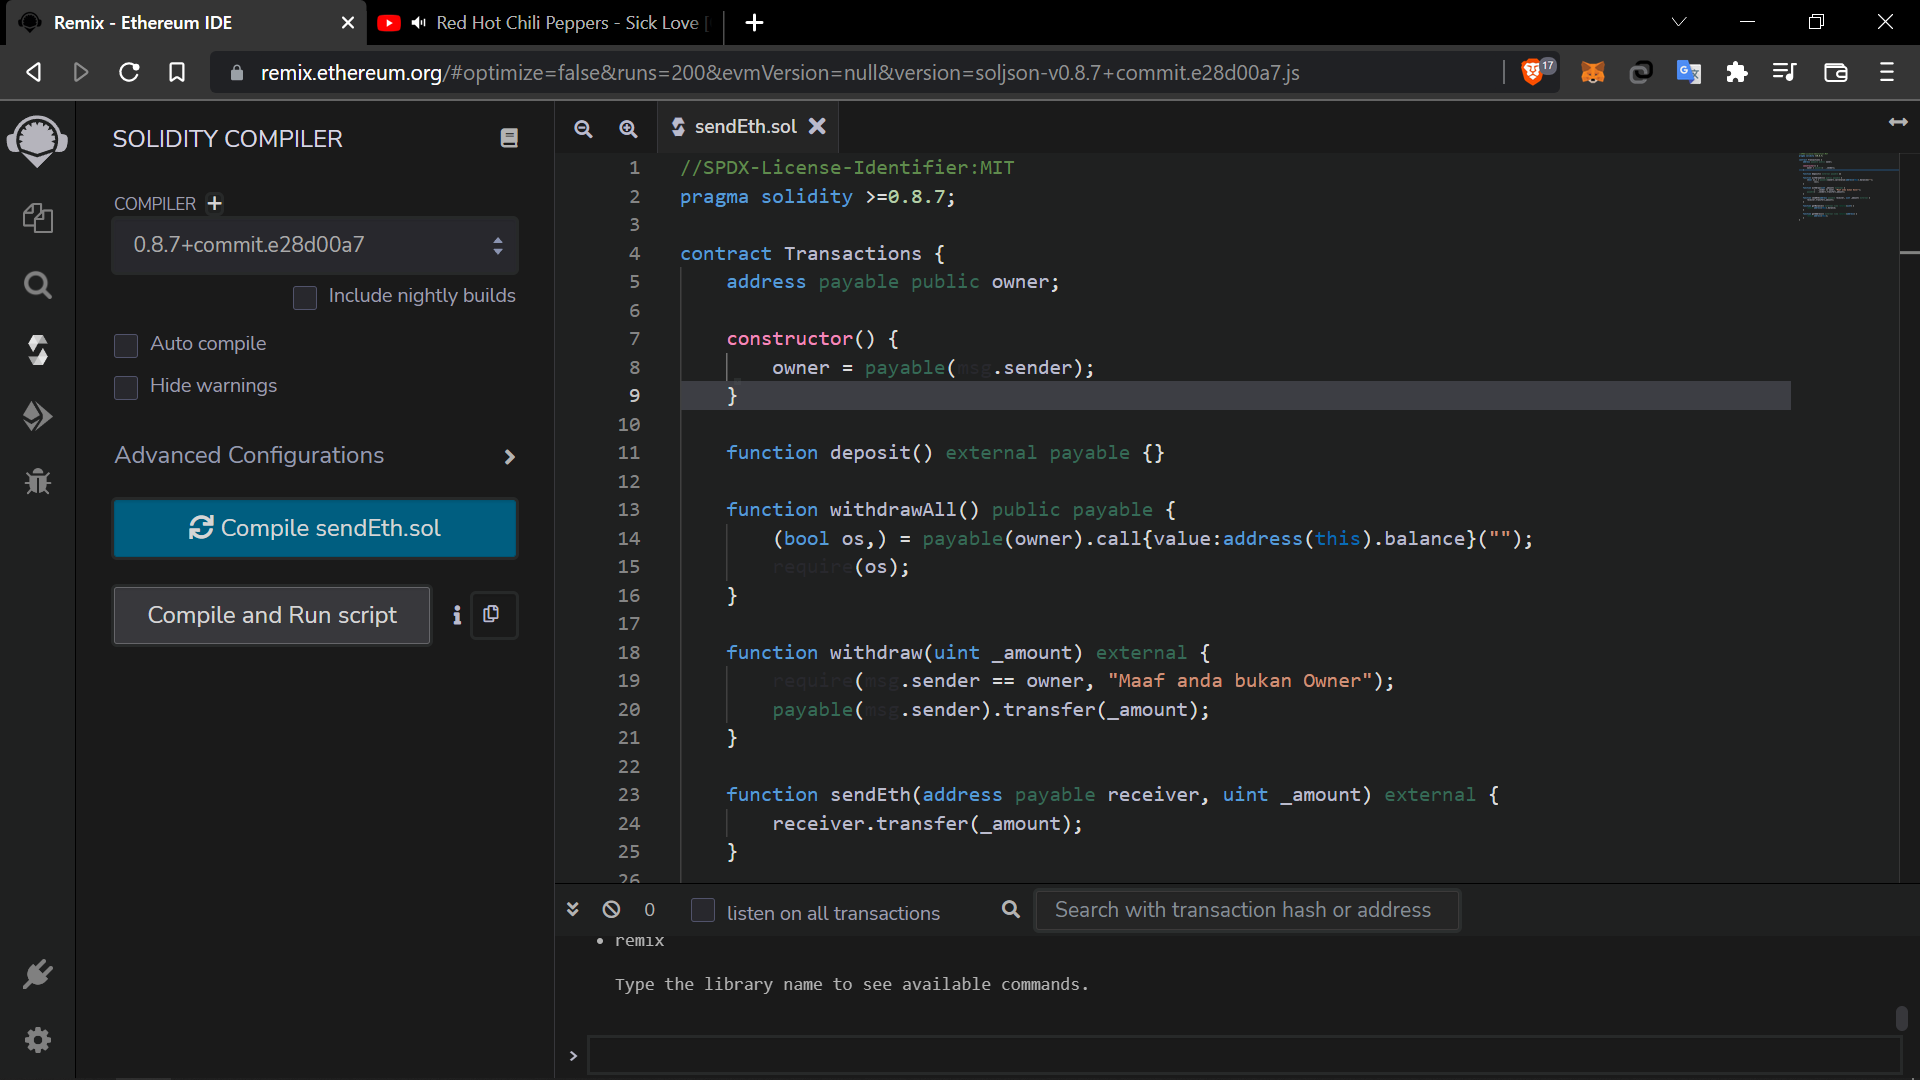
\includegraphics[scale=0.2]{gambar/bab3/deploy/3.png}
		\caption{Compile source code}
		\label{fig:compile}
	\end{figure}
\item{Setelah selesai di-compile, klik Copy ABI kemudian simpan di notes}
	\begin{figure}[htp]
		\centering
		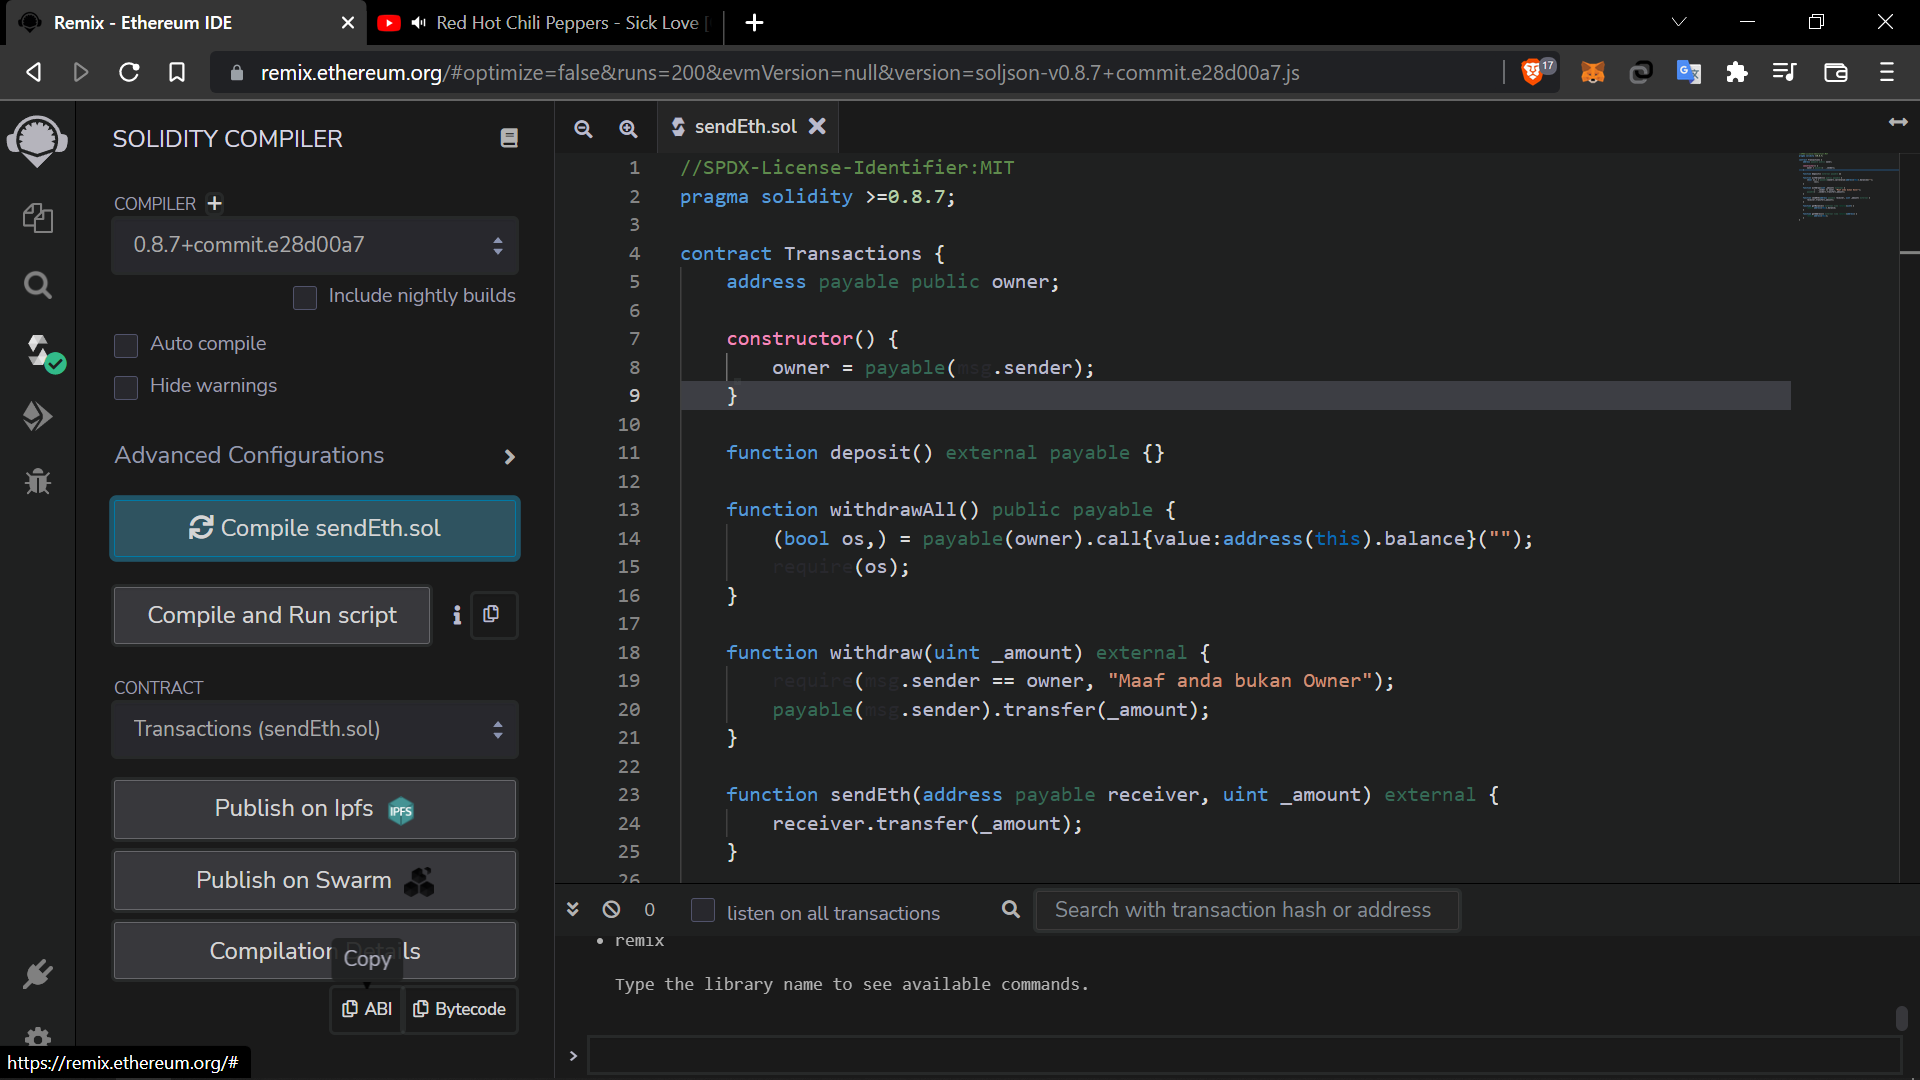
\includegraphics[scale=0.2]{gambar/bab3/deploy/4.png}
		\caption{Mengambil data ABI}
		\label{fig:inputABI}
	\end{figure}
\newpage
\item{Copy ABI ke source code frontend. Masukkan ABI ke dalam variabel baru di file JavaScript dan beri nama nama variabel ABI.}
	\begin{figure}[htp]
		\centering
		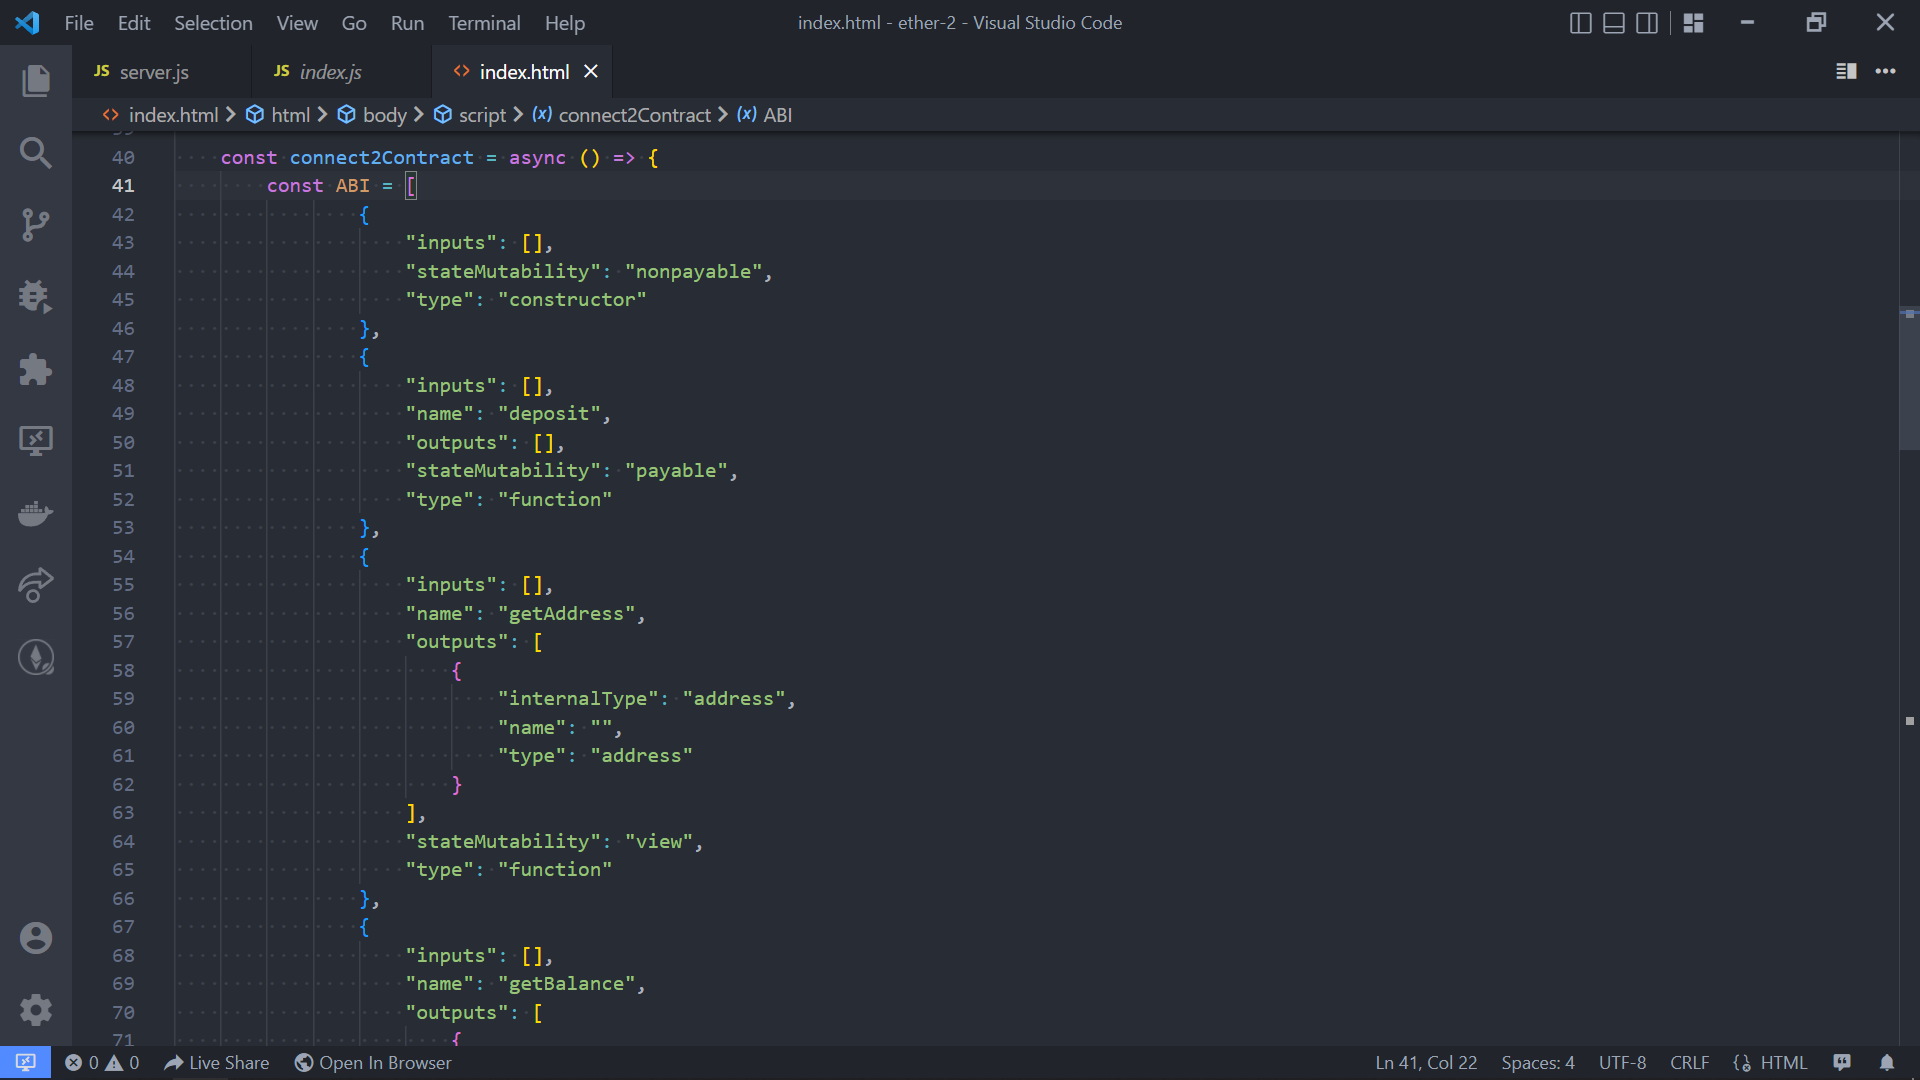
\includegraphics[scale=0.2]{gambar/bab3/deploy/7.png}
		\caption{Memasukkan ABI ke dalam source code frontend}
		\label{fig:abitofront}
	\end{figure}
\end{enumerate}

\subsection{Persiapan Metamask}
\label{subsec:solidityandremix}

Untuk menghubungkan langsung ke jaringan besar Ethereum, penelitian ini akan menggunakan Metamask. Metamask adalah sebuah gateway \emph{Ethereum} yang merupakan sarana utama untuk menghubungkan pengguna ke jaringan \emph{Ethereum} yang kompleks. Dalam Metamask, pengguna memanfaatkan beberapa sub-jaringan yang bisa digunakan maupun jaringan utama \emph{Ethereum} yang bisa digunakan untuk kegiatan di \emph{Ethereum}. Dalam Metamask sendiri semua jaringan yang ada merupakan jaringan Layer 0 yang mana merupakan jaringan yang memiliki harga gas/fee transaction sendiri. Untuk menggunakan Metamask pengguna perlu melakukan setup ke Metamask dan membuat akun dengan membuat dan menghapalkan private key sendiri untuk keamanan akun sendiri. Kemduian di dalam Metamask sendiri untuk melakukan transaksi perlu gas/transaction fee yang merupakan turunan dari \emph{Ether}. Turunan itu merupakan Finney (2$^{-3}$), Scabo (2$^{-6}$), Gwei (2$^{-9}$), Mwei (2$^{-12}$), Kwei (2$^{-15}$), Wei (2$^{-18}$).
\\
\newpage
Pada bagian setup gateway ini, ada beberapa langkah yang perlu dilakukan. Berikut langkah - langkahnya:
\begin{enumerate}
\item{Download Metamask dan Install di web browser pilihan.}
	\begin{figure}[htp]
		\centering
		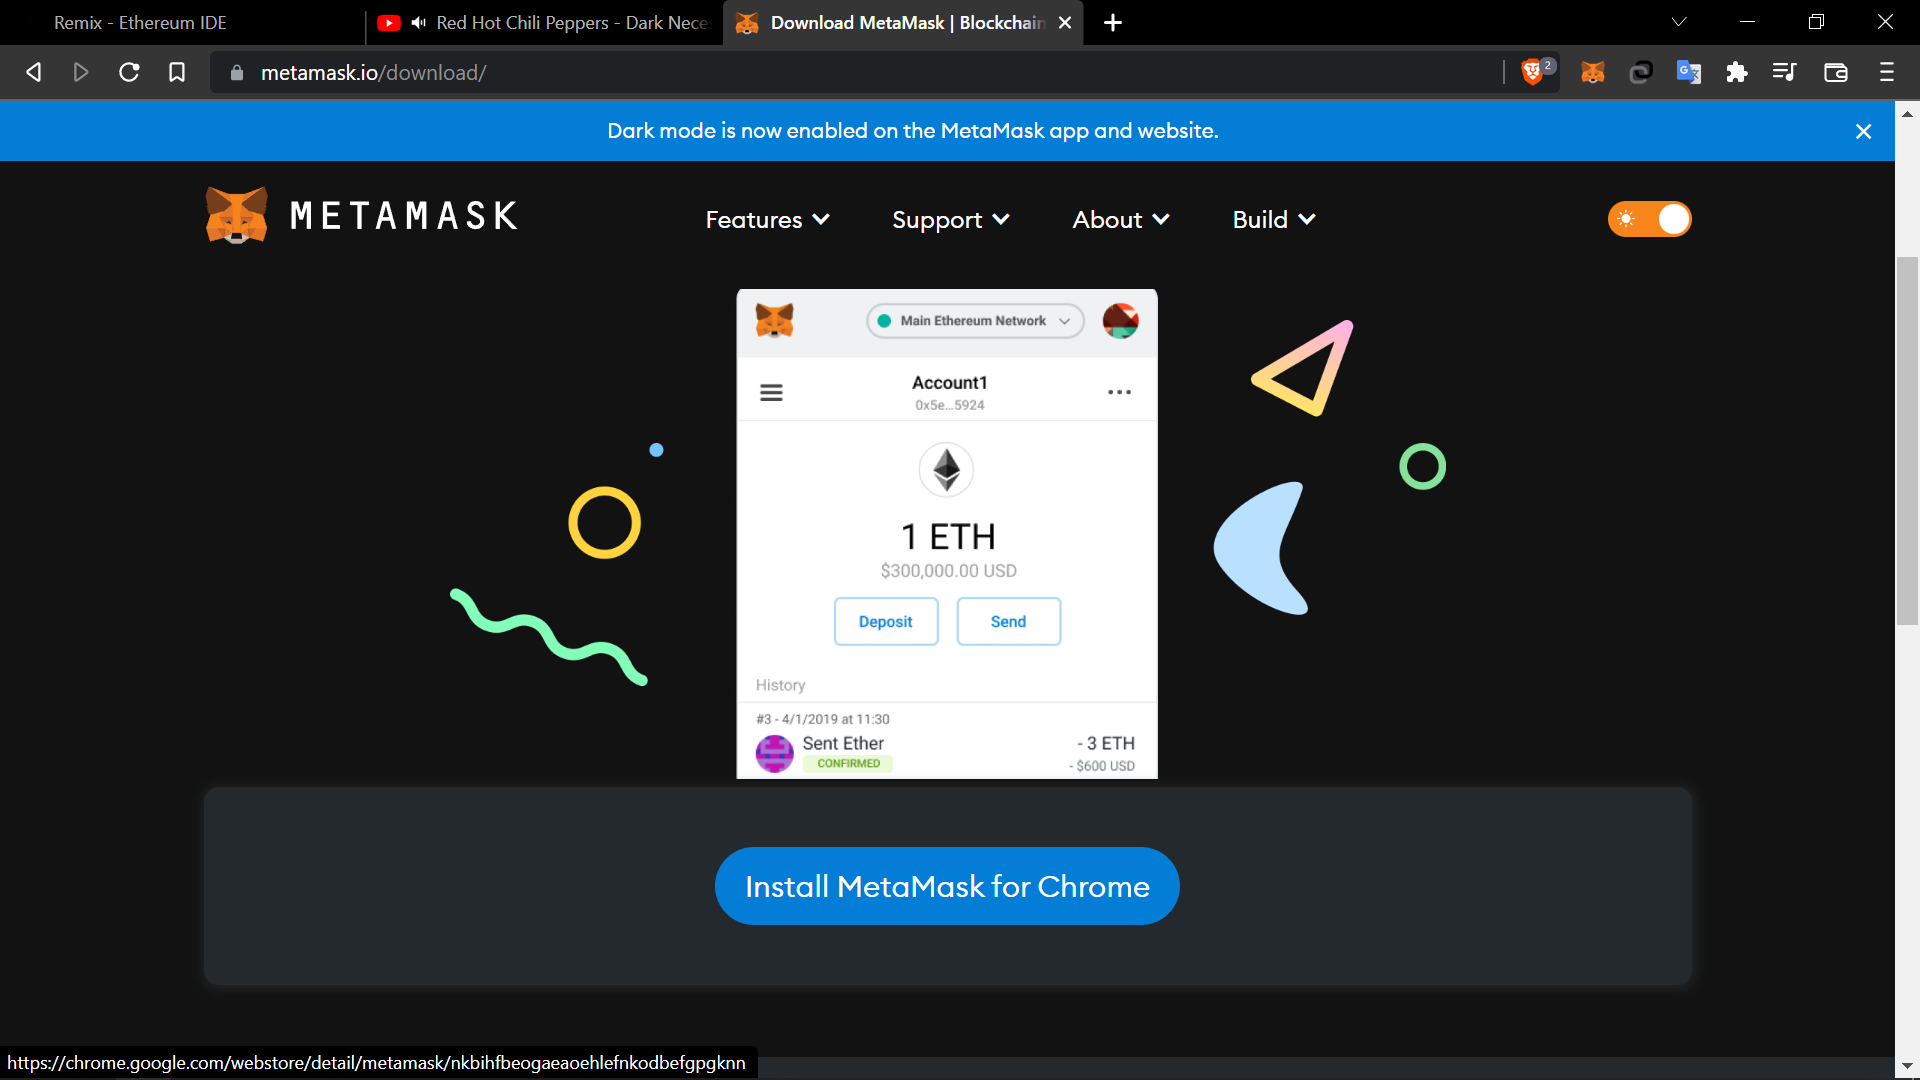
\includegraphics[scale=0.2]{gambar/bab3/metamask/1.png}
		\caption{Download Metamask untuk browser}
		\label{fig:downloadmetamask}
	\end{figure}
\item{Login ke Metamask apabila sudah mempunyai akun. Apabila belum mempunyai akun, buat akun.}
	\begin{figure}[htp]
		\centering
		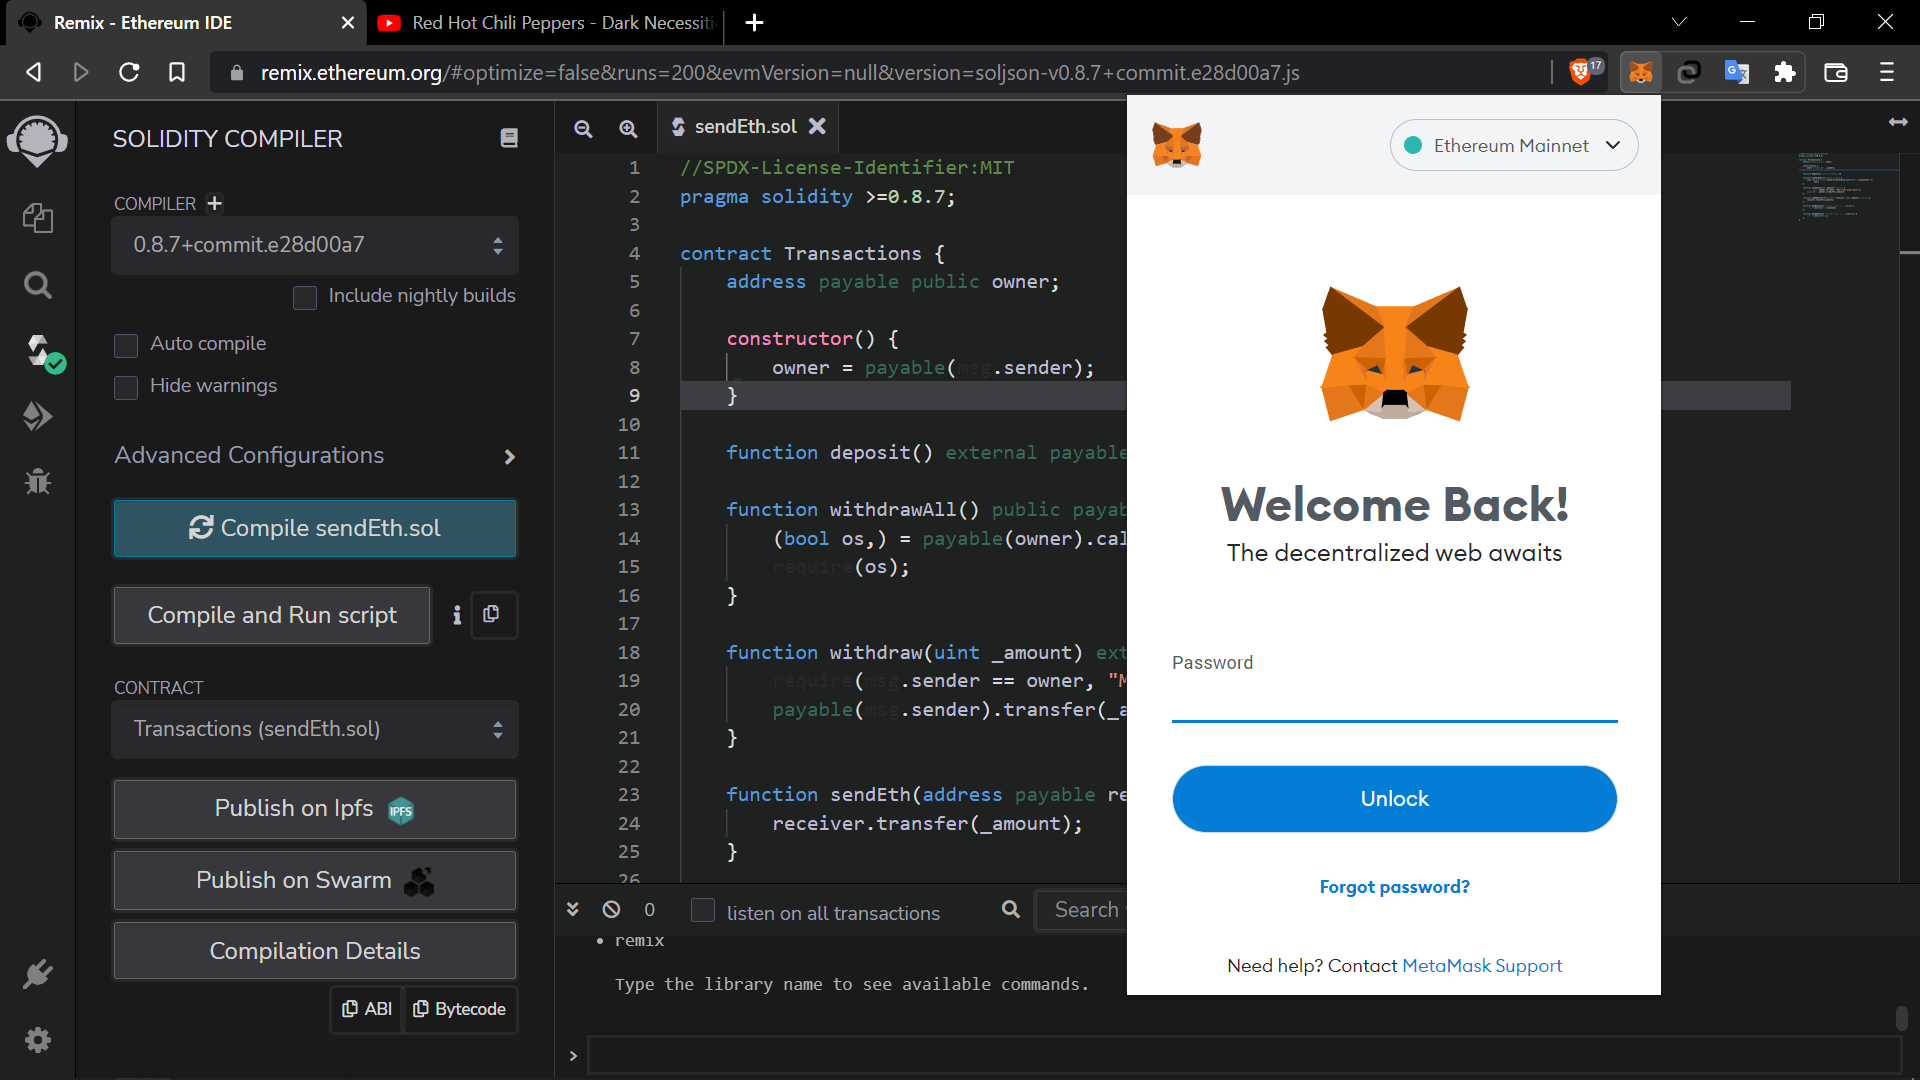
\includegraphics[scale=0.2]{gambar/bab3/metamask/2.png}
		\caption{Log in ke Metamask}
		\label{fig:login2metamask}
	\end{figure}
\item{Setelah login ke Metamask, selanjutnya ke alamat web testnet ETH2.0 di kiln.themerge.dev}
\newpage
\item{Selanjutnya hubungkan Metamask ke testnet yang tersedia.}
	\begin{figure}[htp]
		\centering
		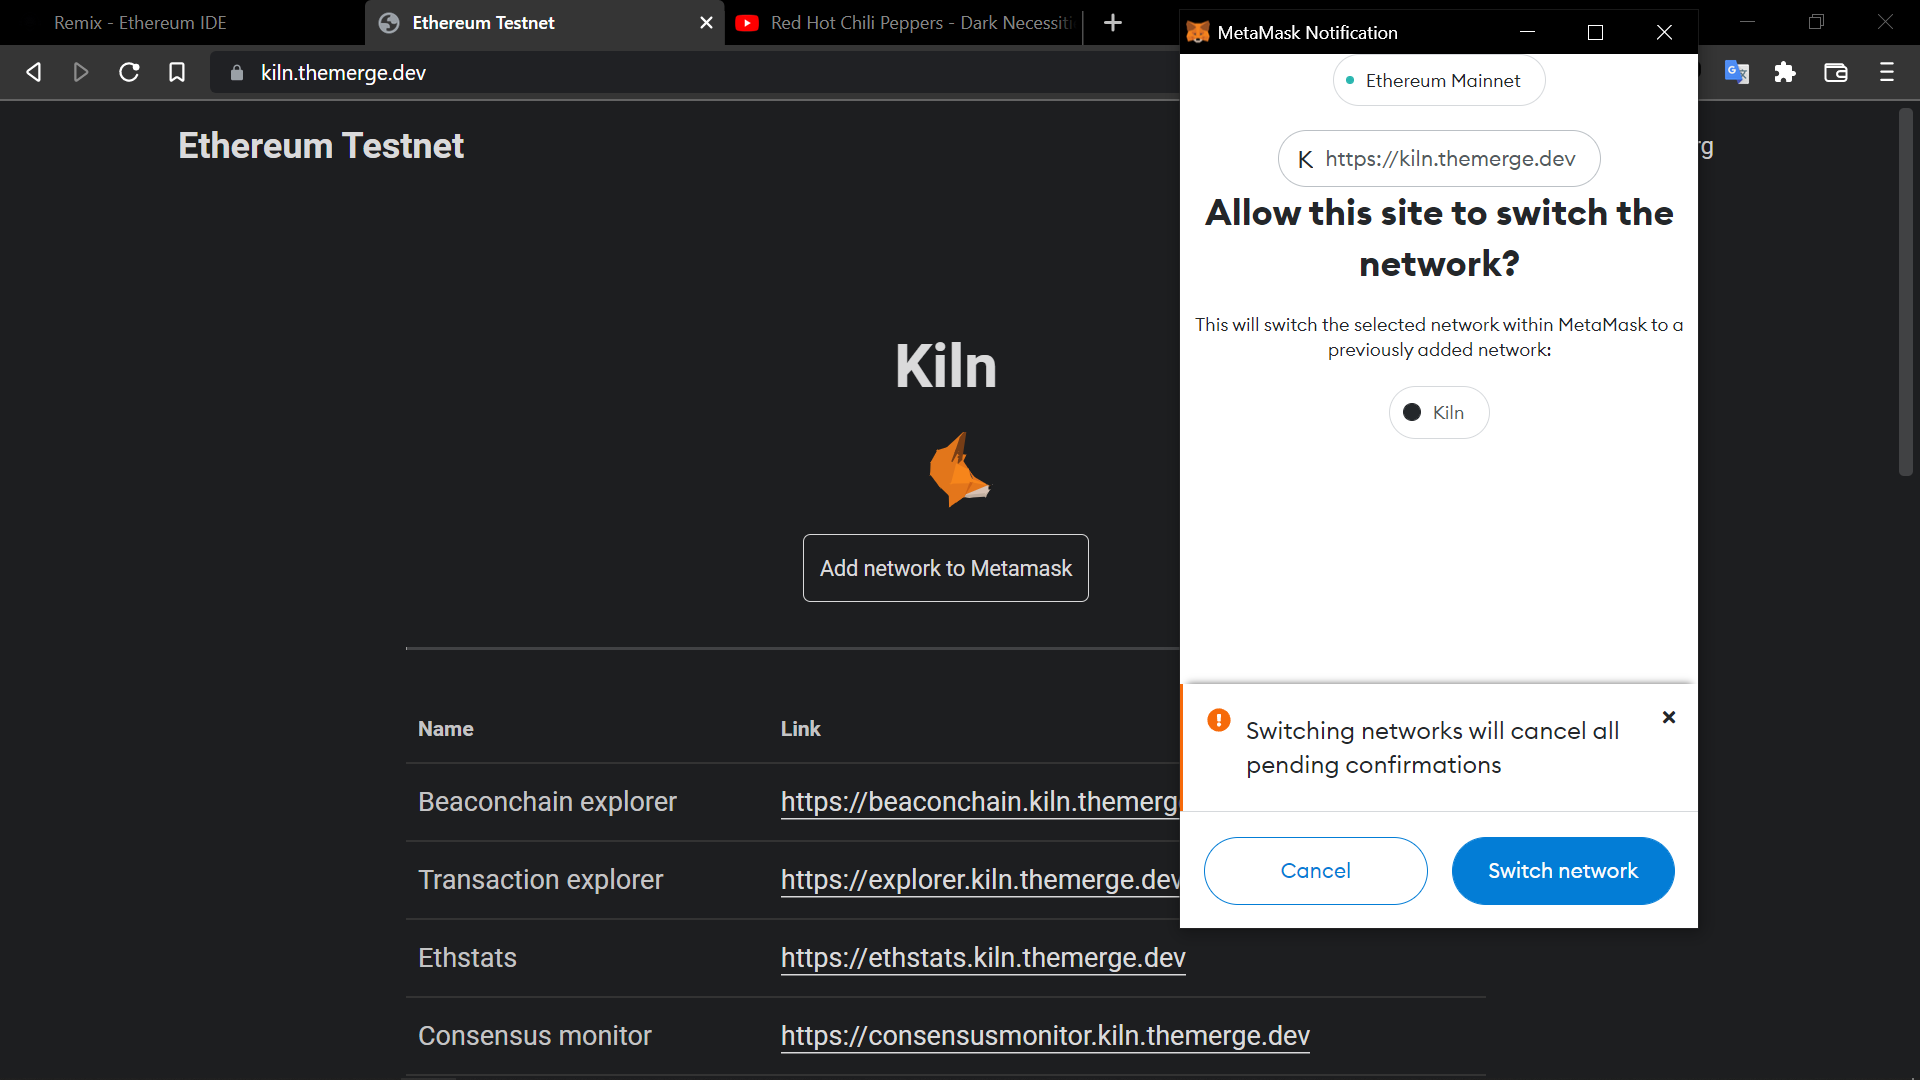
\includegraphics[scale=0.2]{gambar/bab3/metamask/4.png}
		\caption{Menghubungkan ke jaringan testnet ETH2.0}
		\label{fig:connect2testnet}
	\end{figure}
\item{Setelah terhubung ke jaringan testnet, pergi ke faucet resmi jaringan testnet. Faucet ini berguna sebagai tempat mendapatkan Ether yang bersirkulasi di jaringan testnet. Ether ini nantinya digunakan untuk pengujian. Setelah di faucet masukkan address akun kita dan minta dana Ether. Jika sudah selesai, Ether akan masuk ke akun.}
\item{Dapatkan Ether secukupnya}
	\begin{figure}[htp]
		\centering
		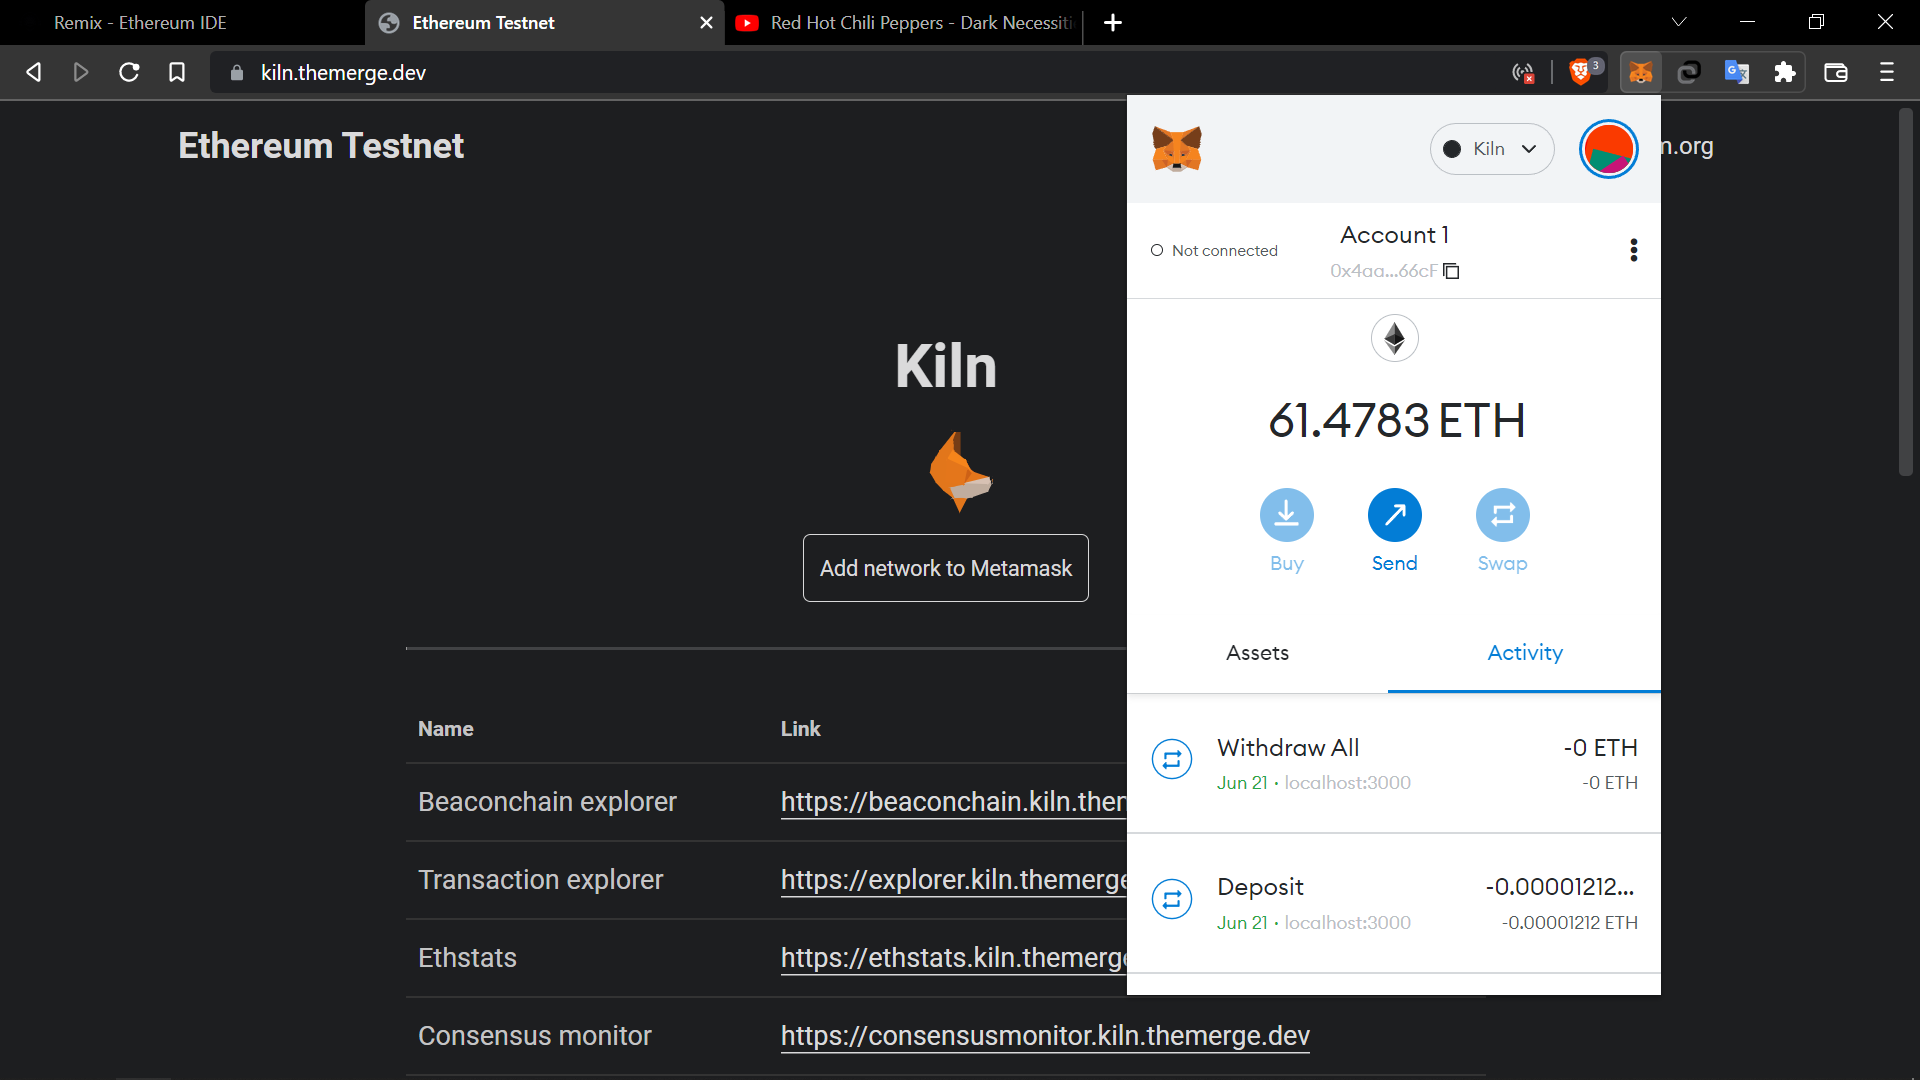
\includegraphics[scale=0.2]{gambar/bab3/metamask/6.png}
		\caption{Metamask siap digunakan}
		\label{fig:accready}
	\end{figure}
\end{enumerate}

\subsection{Frontend/Antarmuka User}
\label{subsec:frontenduser}

Bagian frontend atau biasa dikenal sebagai antarmuka user pada penelitian ini adalah bagian antarmuka tempat user melakukan berbagai interaksi dengan Smart Contract. Ada banyak library maupun framework yang tersedia untuk digunakan sebagai alat untuk membuat antarmuka user berbasis web ini. Salah satu library yang digunakan untuk pembuatan antarmuka user adalah Web3 JavaScript. Web3 JavaScript adalah sebuah API yang digunakan sebagai penghubung antara frontend web dengan smart contract. Web3 ini memungkinkan interaksi dengan smart contract pada pelbagai level dan mengirimkan hasil dari interaksi dengan smart contract dalam bentuk .json ke frontend. Pada Web3 secara umum, mempunyai beberapa fitur dasar untuk menghubungkan ke smart contract yang telah dibuat. Fitur tersebut adalah membuat module untuk Ethereum yang kita pilih, menginisiasi gateway yang digunakan, hingga melakukan transaksi blockchain secara umum.\\
Dalam pembuatan antarmuka untuk user, digunakan Web3 JavaScript untuk menghubungkan antara Smart Contract dengan antarmuka user. Untuk skema pengiriman data ke Smart Contract, frontend menggunakan yaitu Application Binary Interface. Application Binary Interface adalah sebuah interface antara frontend dengan setiap fungsi yang bisa diinteraksikan dalam suatu Smart Contract. ABI ini berberntuk JSON dengan memuat :
\begin{enumerate}
\item{Tipe. Yaitu golongan suatu fungsi bisa berupa 'fungsi','konstruktor', maupun 'terima'}
\item{Nama dari fungsi itu sendiri}
\item{Input yang diterima, baik parameter input maupun tipe input}
\item{Output yang akan dikeluarkan, setiap jenis maupun namanya}
\item{Kendali mutasi dari suatu fungsi. Yaitu kendali yang diberikan untuk berinteraksi mengubah satu maupun lebih variabel dalam suatu fungsi} 
\end{enumerate}
\newpage
Dari ABI ini, kemudian dibuatkan setiap fungsi javascript yang memanggil setiap fungsi yang bisa diinteraksikan. Telah dilakukan pembuatan ABI ke dalam JavaScript. Berikut hasilnya :
	
\begin{figure}[htp]
		\centering
		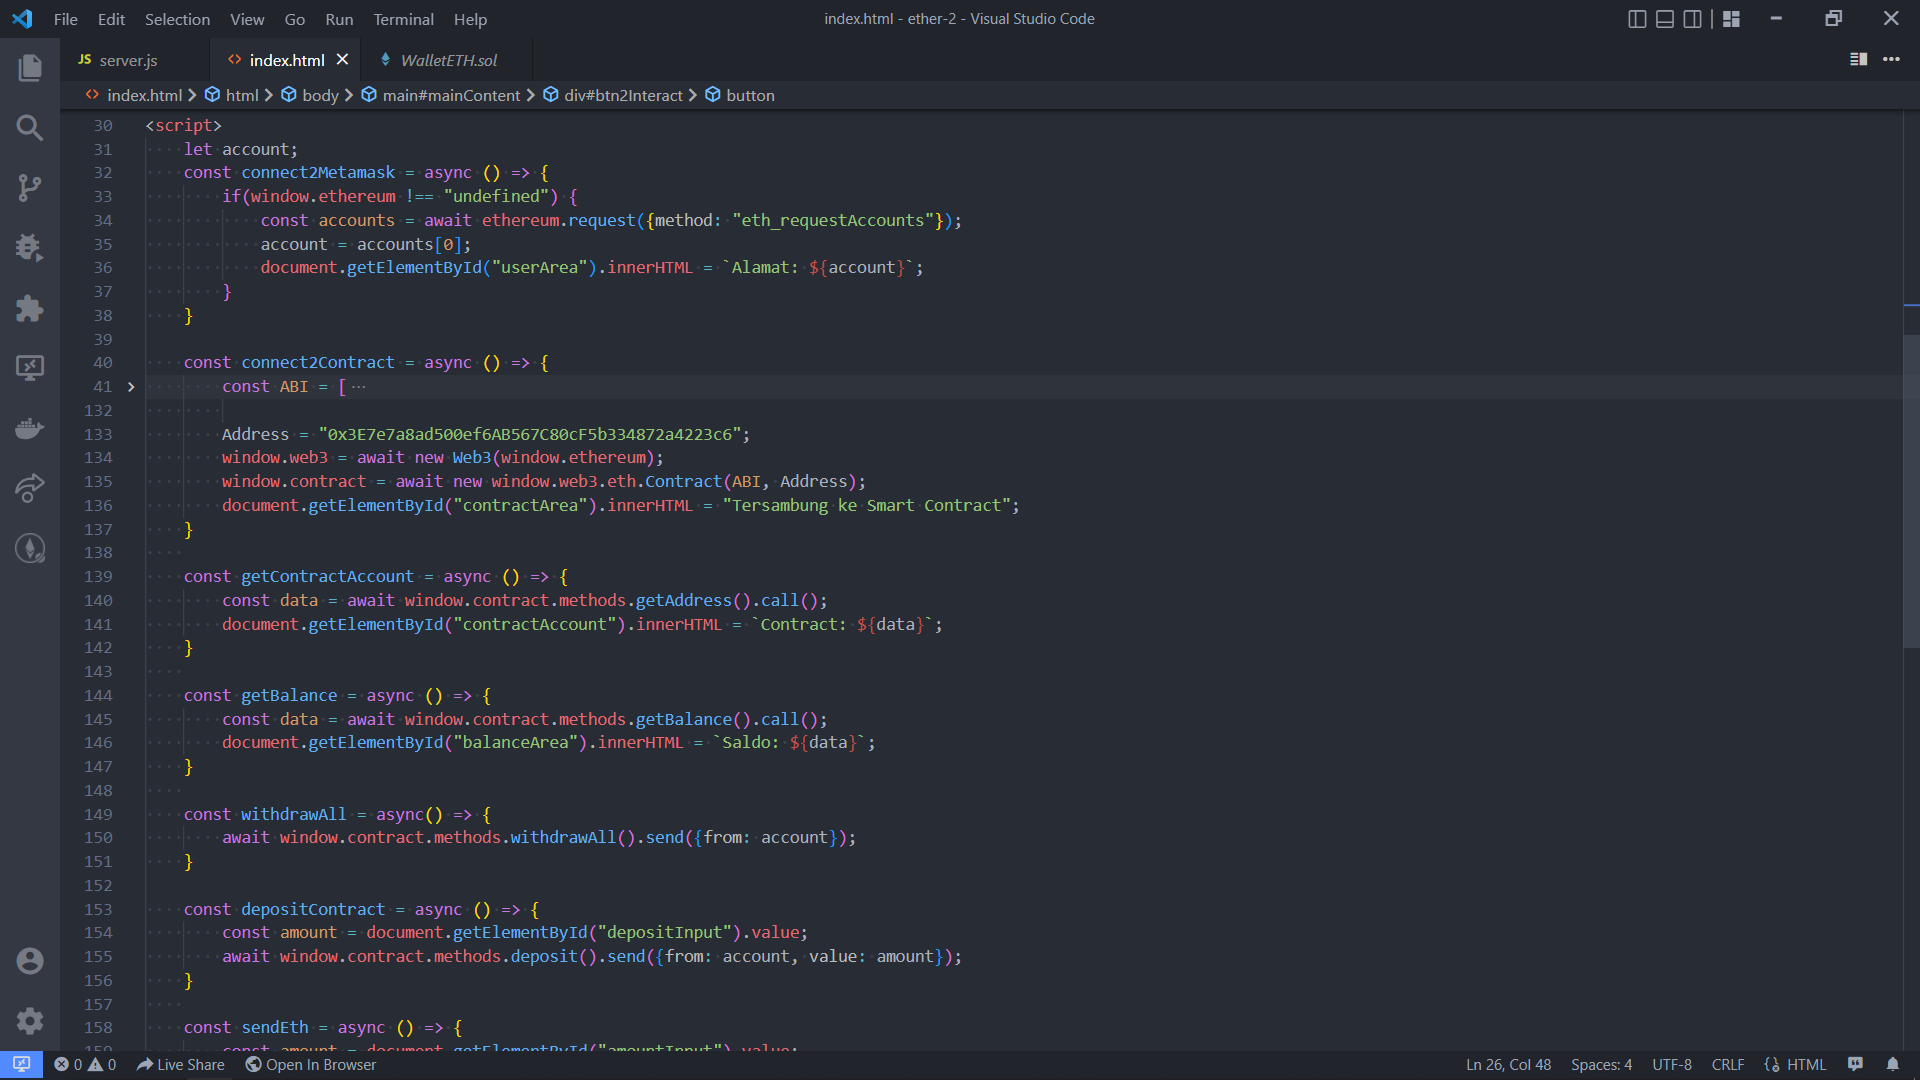
\includegraphics[scale=0.2]{gambar/bab3/front/1.png}
		\caption{Membuat variabel ABI ke dalam frontend (1)}
		\label{fig:abiready}
	\end{figure}

\begin{figure}[htp]
		\centering
		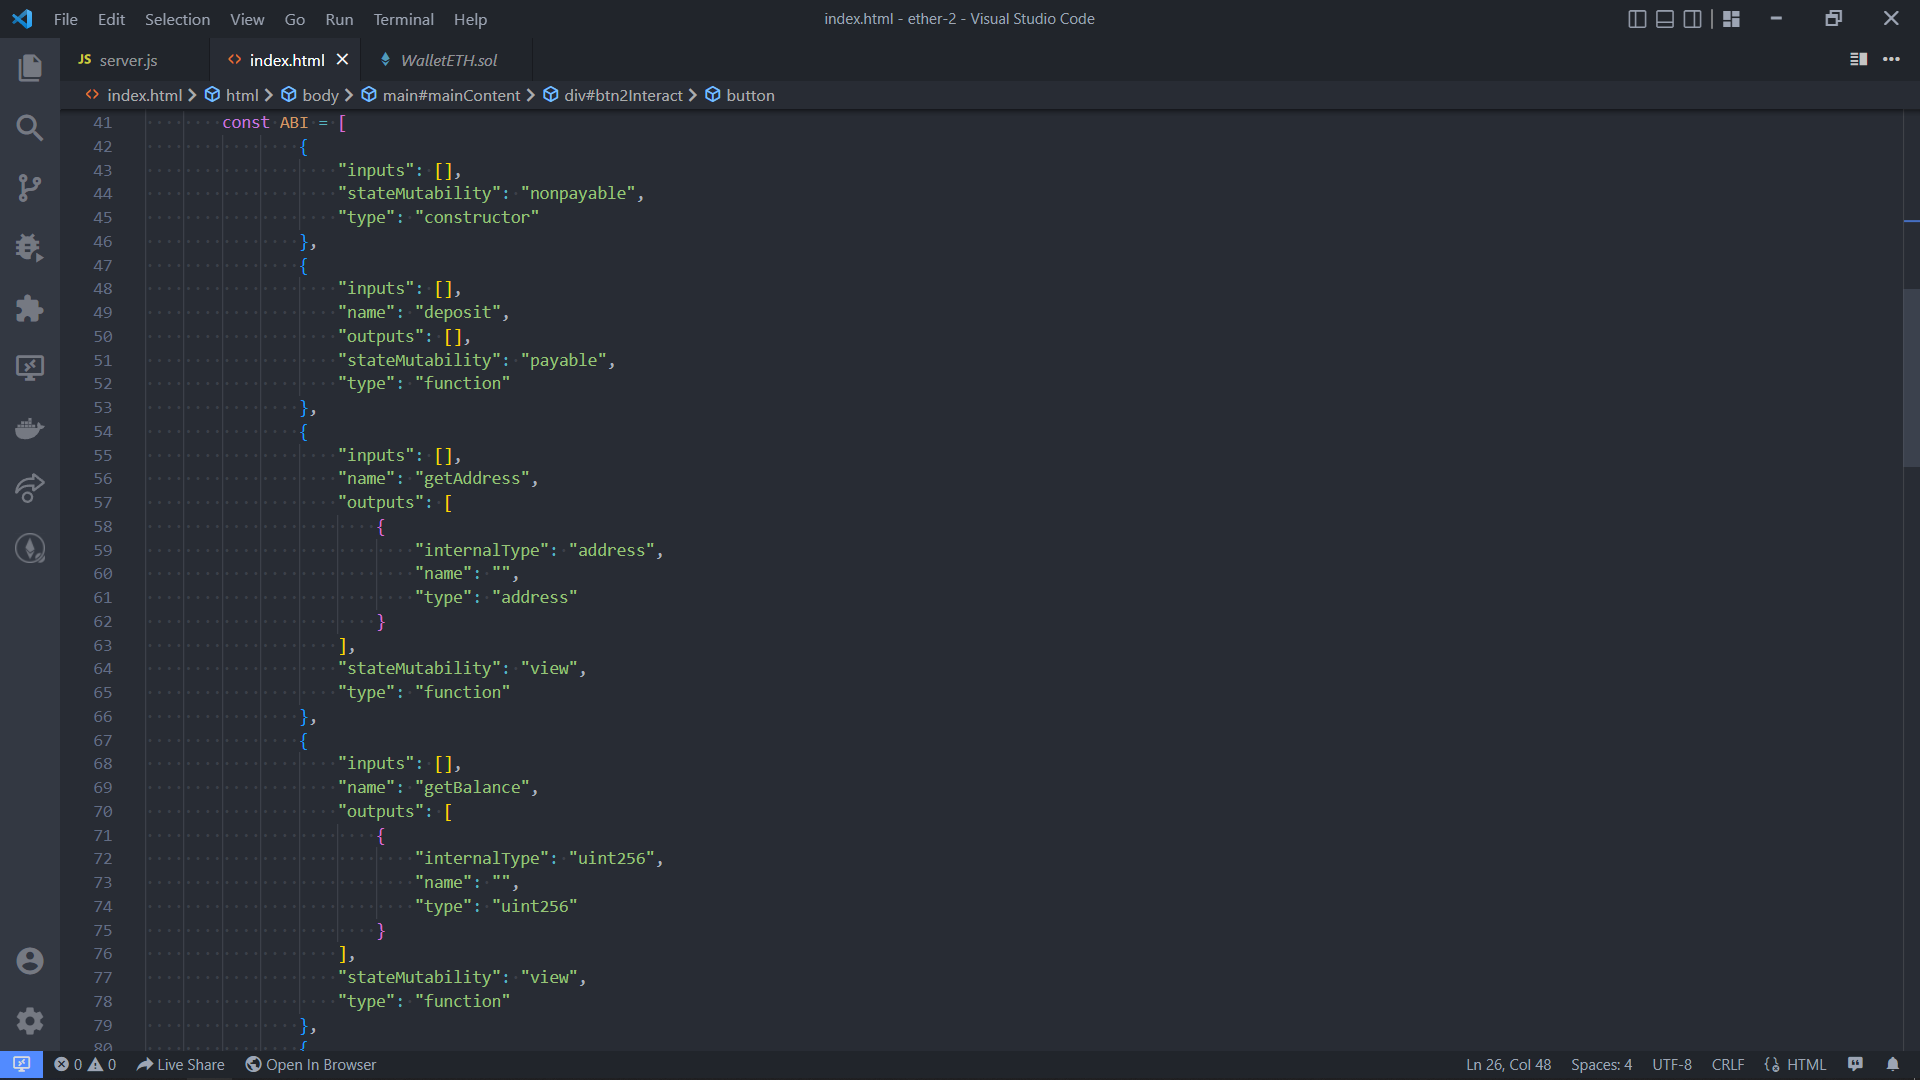
\includegraphics[scale=0.2]{gambar/bab3/front/2.png}
		\caption{Membuat variabel ABI ke dalam frontend (2)}
		\label{fig:abiready2}
	\end{figure}
\newpage
\section{Use Case User}
\label{sec:usecaseuser}

Di bagian antarmuka pengguna, ada beberapa fungsi utama dari penelitian ini yang bisa dilakukan oleh pengguna. Berikut adalah use case dari penggua.
\begin{figure}[htp]
	\centering
	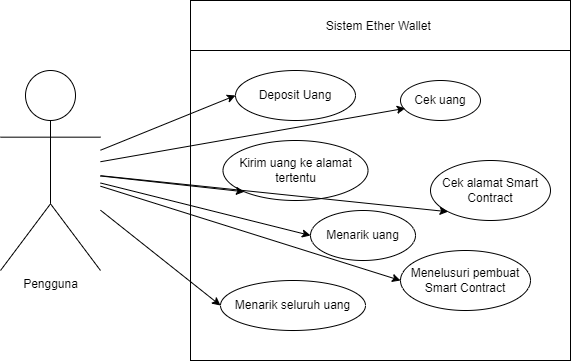
\includegraphics[scale=0.45]{gambar/use-case-diagram-sistem.png}
	\caption{Use Case Diagram antarmuka pengguna}
	\label{fig:usecasefrontend}
\end{figure}

Dari use case diagram diatas, fitur pengguna dapat dijabarkan menjadi berikut:

\begin{itemize}

\item{Deposit Uang}
	\\Deposit uang dari pengguna ke Smart Contract bisa dilakukan melalui gateway Ethereum. Deposit ini menggunakan satuan turunan Ether yaitu Wei. Deposit ke Smart Contract dilakukan untuk menggunakan fitur fitur yang tersedia di Smart Contract ini. Untuk melakukan fitur deposit pengguna bisa mengikut langkah berikut:
\begin{figure}[htp]
	\centering
	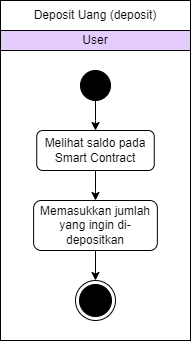
\includegraphics[scale=0.6]{gambar/deposit-diagram.png}
	\caption{Diagram cara deposit}
	\label{fig:diagramdeposit}
\end{figure}

\item{Mengambil Uang}
	\\Untuk fitur mengambil uang, pengguna diberikan dua opsi. Opsi pertama yaitu opsi utnuk mengambil sebagian uang yang telah dideposit ke Smart Contract. Opsi pertama menawarkan berapa banyak uang yang ingin diambil dalam satuan Wei.

\begin{figure}[htp]
	\centering
	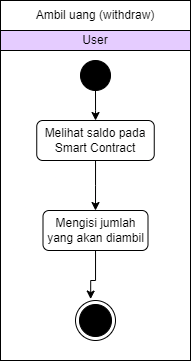
\includegraphics[scale=0.5]{gambar/withdraw-diagram.png}
	\caption{Diagram cara ambil sebagian uang dari Smart Contract}
	\label{fig:diagramwithdraw}
\end{figure}

Untuk fitur kedua yaitu opsi untuk mengambil seluruh uang yang telah dideposikan ke Smart Contract. Opsi ini memungkinkan seluruh uang yang telah dideposit diambil langsung.
\begin{figure}[htp]
	\centering
	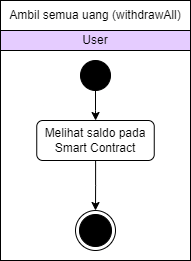
\includegraphics[scale=0.6]{gambar/withdrawAll-diagram.png}
	\caption{Diagram cara ambil seluruh saldo dari Smart Contract}
	\label{fig:diagramwithdrawall}
\end{figure}

\item{Mengirim Uang}
	\\Opsi mengirimkan uang yang telah disimpan di Smart Contract bisa dilakukan dengan mengisi alamat tujuan dan nominal yang dikirimkan dalam satuan Wei:
\begin{figure}[htp]
	\centering
	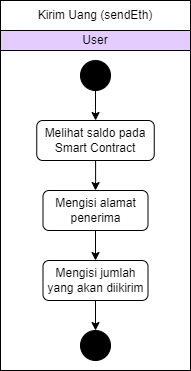
\includegraphics[scale=0.6]{gambar/sendEth-diagram.png}
	\caption{Diagram cara mengirim uang}
	\label{fig:diagramsendeth}
\end{figure}
\end{itemize}

  \cleardoublepage

  % Bab 4 pengujian dan analisis
  \chapter{HASIL DAN PEMBAHASAN}
\label{chap:hasilpembahasan}

Pada bab sebelumnya telah dibuat penjelasan mengenai sistem penelitian secara keseluruhan. Mulai dari bagian antarmuka pengguna, hingga bagian smart contract telah dibuat dan didokumentasikan. Setelah itu pada bagian ini akan dijelaskan pengujian yang akan dilakukan pada sistem. Pengujian bertujuan untuk menguji apakah seluruh fitur yang akan dibuat berjalan sesuai dengan tujuan penelitian ini.

\section{Skenario Pengujian}
\label{sec:skenariopengujian}

Pada bagian pengujian, akan dilakukan pengujian sistem secara menyeluruh. Pengujian ini mencakup bagian antarmua pengguna dan fitur Smart Contract yang telah di-deploy.Pengujian ini nantinya akan dilakukan di beberapa perangkat yang telah disebutkan pada bab sebelumnya dengan variabel yang berbeda. \\
Pengujian bagian pertama adalah pengujian antarmuka pengguna apakah sudah memenuhi kebutuhan sesuai prosedur yang ditetapkan. Tujuannya agar fitur yang dibuat sudah sesuai dengan penjelasan dan use case sesuai pada bab sebelumnya.
Pengujian kedua adalah pengujian fitur Smart Contract yang merupakan pengujian berbagai fungsi yang telah ditetapkan di awal penelitian. Apakah dapat berjalan sesuai dengan ekspektasi penelitian ini.\\
Berikut adalah pengujian yang telah dilakukan.

\subsection{Pengujian Antarmuka Pengguna}
\label{subsec:ujiuiux}

Pada bagian ini pengujian antarmuka pengguna dilakukan dengan menggunakan metode Black Box testing. Black Box testing dipilih pada pengujian karena Black Box testing merupakan metode pengujian suatu aplikasi dari sisi penggunanya sendiri. Artinya pada pengujian ini, diharapkan pengujian dapat menempatkan posisinya sebagai pengguna aplikasi ini. Pada

\subsection{Pengujian Pada Jaringan Tes Kintsugi}
\label{subsec:teskintsugi}

Berikut adalah hasil pengujian pada jaringan tes PoS Kintsugi.

\begin{longtable}{|c|c|c|}
  \caption{Hasil Pengujian Pada Jaringan Kintsugi}
  \label{tb:kintsugitest}\\
  \hline
  \rowcolor[HTML]{C0C0C0}
  \textbf{Nomor} & \textbf{User 1} & \textbf{User 2} \\
  \hline
  1 & Sukses & Sukses \\
  2 & Sukses & Sukses \\
  3 & Sukses & Sukses \\
  \hline
\end{longtable}

Sembari melakukan transaksi dilakukan pengukuran durasi setiap transaksi yang telah sukses

\begin{longtable}{|c|c|}
  \caption{Hasil Pengukuran Durasi Transaksi di Jaringan Tes Kintsugi}
  \label{tb:kintsugispeed}\\
  \hline
  \rowcolor[HTML]{C0C0C0}
  \textbf{Nomor} & \textbf{Kecepatan} \\
  \hline
  1 & 20,27 detik  \\
  2 & 26,57 detik\\
  3 & 35,07 detik \\
  \hline
\end{longtable}

\subsection{Pengujian Pada Jaringan Tes Kiln}
\label{subsec:teskiln}

Berikut adalah hasil pengujian pada jaringan tes PoS Kintsugi.

\begin{longtable}{|c|c|c|}
  \caption{Hasil Pengujian Deployment Smart Contract Pada Jaringan Kiln}
  \label{tb:kilntest}\\
  \hline
  \rowcolor[HTML]{C0C0C0}
  \textbf{Nomor} & \textbf{Status}\\
  \hline
  1 & Sukses \\
  2 & Sukses \\
  3 & Sukses \\
  4 & Sukses \\
  5 & Sukses \\
  6 & Gagal \\
  7 & Sukses \\
  \hline
\end{longtable}

Setelah transaksi dapat terjadi dilakukan pengukurang durasi 

\begin{longtable}{|c|c|}
  \caption{Hasil Pengukuran Durasi Deployment Smart Contract di Jaringan Tes Kiln}
  \label{tb:kilnspeed}\\
  \hline
  \rowcolor[HTML]{C0C0C0}
  \textbf{Nomor} & \textbf{Kecepatan} \\
  \hline
  1 & 13,33 detik \\
  2 & 13,33 detik \\
  3 & 13,33 detik \\
  4 & 13,33 detik \\
  5 & 13,33 detik \\
  6 & 13,33 detik \\
  7 & 13,33 detik \\
  \hline
\end{longtable}
  \cleardoublepage

  % Bab 5 penutup
  \chapter{PENUTUP}
\label{chap:penutup}

% Ubah bagian-bagian berikut dengan isi dari penutup

\section{Kesimpulan}
\label{sec:kesimpulan}

Berdasarkan hasil pengujian yang telah dilakukan, dapat ditarik kesimpulan sebagai berikut :

\begin{enumerate}[nolistsep]

  \item Pembuatan Dompet Digital menggunakan Ethereum dapat dilakukan dengan pembuatan sistem smart contract kemudian menghubungkannya ke website yang telah dibuat.

\end{enumerate}

\section{Saran}
\label{chap:saran}

Untuk pengembangan sistem dompet digital lebih lanjut terdapat beberapa bagian yang bisa direvisi antara lain:

  \cleardoublepage

  % Daftar pustaka
  \renewcommand\bibname{DAFTAR PUSTAKA}
  \addcontentsline{toc}{chapter}{\bibname}
  \bibliographystyle{apacite}
  \bibliography{pustaka/pustaka.bib}
  \cleardoublepage

  % Biografi penulis
  \begin{center}
  \Large
  \textbf{BIOGRAFI PENULIS}
\end{center}

\addcontentsline{toc}{chapter}{BIOGRAFI PENULIS}

\vspace{2ex}

\begin{wrapfigure}{L}{0.3\textwidth}
  \centering
  \vspace{-3ex}
  % Ubah file gambar berikut dengan file foto dari mahasiswa
  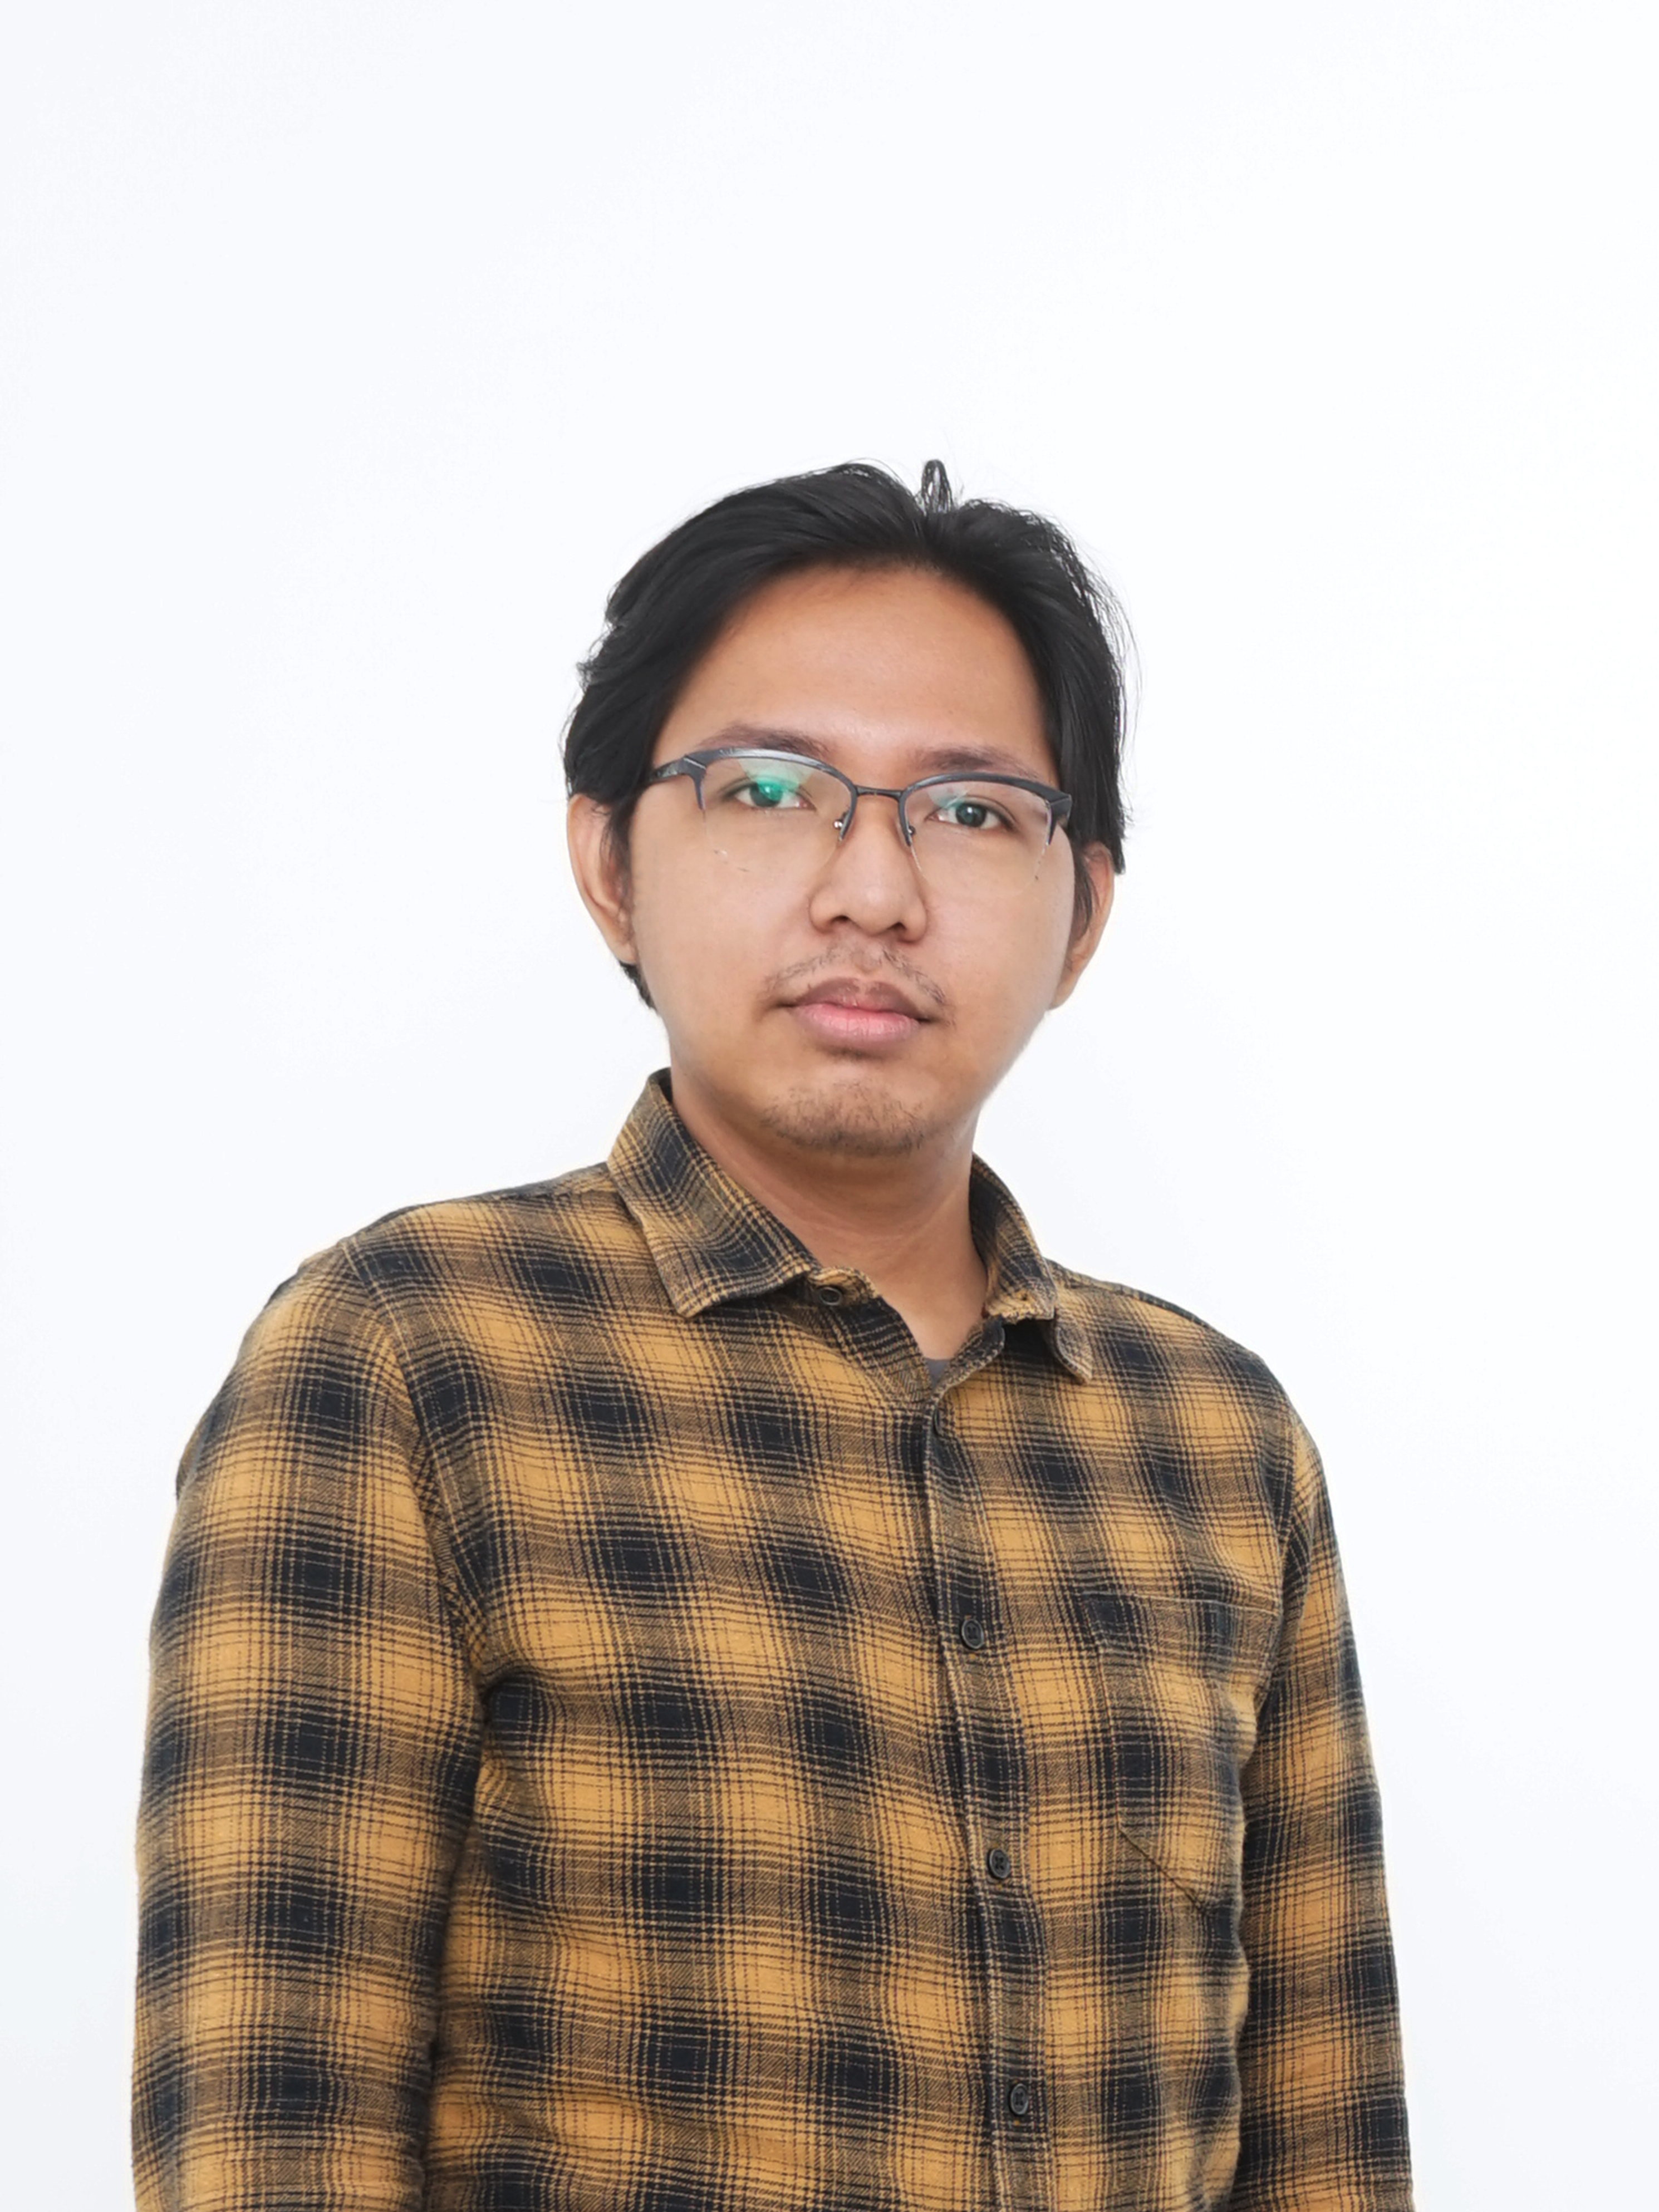
\includegraphics[width=0.3\textwidth]{gambar/dimas.jpg}
  \vspace{-4ex}
\end{wrapfigure}

% Ubah kalimat berikut dengan biografi dari mahasiswa
Dimas Nazli Bahaduri, lahir pada 20 Mei 2000 adalah anak terakhir dari tiga bersaudara dari Ibu Kusmiati dan Alm. Abdul Rauf. Dimas Nazli Bahaduri adalah anak yang pendiam sejak lahir dan suka melakukan perincian bahkan merusak berbagai benda-benda di sekitarnya hanya untuk keingintahuannya. Merasa tertarik dengan dunia yang imajiner, dia memiliki hobi menggambar dan melebar ke berbagai bentuk seni gerak, suara, hingga citra. Selain memiliki hobi yang bersinggungan dengan dunia seni, dia juga suka untuk mempertanyakan  sekitar berkat ketidak-sengajaannya membaca Kongzi. Salah satu ajaran yang digaungkan kembali oleh Kongzi adalah sadar untuk menjadi siapa dan seutuhnya menjadi sesuai kemampuannya. Maka dari itu Dimas bercita cita mempunyai studio Animasi untuk anak anak bertalenta dan menimba ilmu sebanyak dan sekomprehensif mungkin. Semua itu berangkat dari momen abangnya yang berkuliah selama 3 tahun dan lulus pada tahun 2006 dari sekolah kedinasan. 
\\Rejeki pun menempatkan Dimas di Insitut Teknologi Sepuluh Nopember di jurusan Teknik Komputer.Mengenyam bangku perguruan tinggi membuka pandangan baru seorang Dimas dan berkontribusi mengasah potensi, kemampuan, dan keinginannya. Melalui berbagai kegiatan organisasi hingga UKM telah ia coba. Ditambah dengan antusiasme dia kepada komputer dan seni digital membuat dia semakin yakin untuk berkuliah di Teknik Komputer ITS. Setelah menempuh kuliah 3.5 tahun lebih di Teknik Komputer menambah pengetahuan dan arti terjatuh, terbangun, senang, susah, kebingungan, hingga bersyukur. Tentu dia merasa beruntung dan bersyukur karena bertemu dosen, tenaga pendidik, staff, teman, kakak tingkat, hingga warga sekitar. Meskipun suatu saat dia tidak akan selamanya di Teknik Komputer,dia merasakan dampaknya dan kebajikan yang dia dapatkan akan dituang di kehidupan selanjutnya. 


  \cleardoublepage

\end{document}
